\subsection{Background}\label{subsec:SAT_background}

  \paragraph*{Representing integers with list of booleans}
    SAT problems are based only on boolean variables. 
    Hence, one of the issues is that we have to represent positive integer numbers. 
    One-hot encoding is a possible solution for representing integers using only boolean variables.\\
    \textit{How does one-hot encoding work?}\\
    For every integer variable we declare one boolean variable for every item of the domain of 
    the numeric variable. Only one boolean per integer variable is set to \texttt{True}. The only \texttt{True} 
    variable corresponds to the value of the domain that is being represented.\\

    This solution leads to a simple implementation of the operations but is not very efficient 
    because it requires the SAT solver to manage a very big quantity of variables and clauses.
    We decided to use decimal-to-binary encoding. \\
    
    Let \(domain\_max\) be the maximum value of the domain of a positive integer variable. 
    The number of boolean variables allocated to represent it is:
    \begin{equation*}
        var\_size = \lceil \log_2 (domain\_max + 1)\rceil
    \end{equation*}
    We have a list of boolean variables that take the value of the corresponding bit of the binary encoding
    of the positive integer. We implemented specific functions to perform mathematical operations.
    They are discussed in Section \ref{subsec:SAT_predicates}.

  \paragraph*{Implementation of the Models}
    We decided to create a default abstract model that has the common parts needed by
    every concrete model. The abstract model is extended by the Base model and the Rotation model. 
    The details of the Rotation model are discussed in Section \ref{subsec:SAT_rotation}\\

    In order to implement the SAT formulation we have used the solver called \texttt{z3}.

% % % % % % % % % % % % % % % % % % % % % % % % % % % % % % % % % % % % % % % % % % % % % % % % % %

\subsection{Variables}\label{subsec:SAT_variables}
  The variables for the SAT solver are lists of boolean variables but their meaning does not differ
  from the definitions in \ref{sec:shared_variables}.
  The size of the lists is calculated to be minimal but safe against overflows of the possible operations.
  \begin{equation*}
    x\_domain\_size = \lceil \log_2 (width - \min_{0 \leq i < nc} (w_i) + \max_{0 \leq i < nc}(w_i) + 1) \rceil
  \end{equation*}
  \( x\_domain\_size \) is the length of each \(x_i\) list of booleans.
  \begin{equation*}
    y\_domain\_size = \lceil \log_2 (max\_makespan - \min_{0 \leq i < nc} (h_i) + \max_{0 \leq i < nc}(h_i) + 1) \rceil
  \end{equation*}
  \(y\_domain\_size\) is the length of each \(y_i\) list of booleans.

  % Several variables are used only locally in functions: they are defined there.\\

% % % % % % % % % % % % % % % % % % % % % % % % % % % % % % % % % % % % % % % % % % % % % % % % % %

\subsection{Predicates and Functions}\label{subsec:SAT_predicates}
  We created several support functions for dealing with the conversion from integers to lists of
  boolean variables and back.\\
  
  If an integer value is provided than it is converted to a list of python \texttt{bool} variables
  that are consistent with 
  \texttt{z3 Bool} variables and can be used to perform calculations.\\
  In this way we achieve the transparency of the mathematical functions for the type of operand 
  used.\\
  The length of the lists of booleans is calculated upon the maximum value of the domain of the
  variable. Padding of the shortest list is performed if necessary in case of operations between
  two values of different domain sizes.

  \paragraph*{All the bits of a list set to False}
    \begin{equation*}
      all\_F(list) = \bigwedge_{b \in list}\neg \ b
    \end{equation*}
  
    \paragraph*{At least one bit of a list must be set to True}
    \begin{equation*}
      at\_least\_one(list) = \bigvee_{b \in list} b
    \end{equation*}

  \paragraph*{At most one} \hfill \\
  %\texttt{\textbf{at\_most\_one(list):}}\\
    We implemented the Heule encoding making this a recursive function.\\
    The base case of the recursion is if the list has less than four elements. In this case the 
    pair-wise encoding is used to calculate the result.\\

    Let n be the length of \(list\) 
    \begin{equation*}
            (n < 4) \Longrightarrow at\_most\_one(list) = \bigwedge_{0 < i < n} \ \ \bigwedge_{i+1 \leq j \leq n}\neg \ (b_i \land b_j)
    \end{equation*}
    In the recursive case we split \(list\)  into two parts: \(list_A\)  has length two, \(list_B\)  is
    the remainder. We introduce a new variable \(y\). We append \(y\)  to \(list_A\)  and ¬\( y\)  to 
    \(list_B\). We than calculate the result through recursion:
    \begin{equation*}
        (n \geq 4) \Longrightarrow at\_most\_one(list) = at\_most\_one(list_A) \land at\_most\_one(list_B)
    \end{equation*}

    We chose this encoding because it achieves a number of clauses of \(3n - 6\)  using \((n-3)/2\) new variables.

  \paragraph*{Exactly one}
    \begin{equation*}
      exactly\_one(list) = at\_most\_one(list) \land at\_least\_one(list)
    \end{equation*}

  \paragraph*{Not equal} \hfill \\
  We must consider the cases where the two lists have different lengths.
  Let \(min\_len\)  be the minimum between the length of the lists, \(exc_1\)  be the part of \(l1\) 
  exceeding \(min\_len\)  and \(exc_2\)  be the part of \(l2\)  exceeding \(min\_len\). At least one 
  among \(exc_1\)  and \(exc_2\)  will be an empty list and will provide no clauses.\\
  \begin{equation*}
    ne(l1, l2) = at\_least\_one(exc_1) \lor at\_least\_one(exc_2)\ \lor \bigoplus_{i \leq min\_len}(l1_i, l2_i)
  \end{equation*}

  \paragraph*{Equal} \hfill \\
    One of the lists is eventually padded with bits set to \texttt{False} than we can
    calculate the result:
    \begin{equation*}
      eq(l1, l2)\ =\ \bigwedge_{0 \leq i < n} \neg\ (l1[i] \oplus l2[i])
    \end{equation*}

  \paragraph*{Greater than or equal} \hfill \\
    We must consider the cases where the two lists have different lengths.
    Let \(min\_len\)  be the minimum between the length of the lists, \(exc_1\)  be the part of \(l1\)  
    exceeding \(min\_len\)  and \(exc_2\)  be the part of \(l2\)  exceeding \(min\_len\). At least one among
    \(exc_1\)  and \(exc_2\)  will be an empty list and will provide no clauses.\\
    \begin{equation*}
          gte(l1, l2) = at\_least\_one(exc_1) \lor ( all\_F(exc_2) \land gte\_same\_len(l1\_cut, l2\_cut))
    \end{equation*}
    Where \(l1\_cut\)  and \(l2\_cut\)  are the result of pruning \(l1\)  and \(l2\)  at length \(min\_len\).\\

  \paragraph*{Greater than or equal of numbers represented with the same quantity of bits} \hfill \\
    The encoding used is the AND encoding with Common Subexpression Elimination as described in 
    \cite{Elgabou} and \cite{Zhao}.\\
    
    Given \(n\) as the length of the lists \(l1\) , \(l2\), we have for the case \(n = 1\):
    \begin{equation*}
      gte\_same\_len(l1, l2) = l1_0 \lor \neg \ l2_0
    \end{equation*}

    otherwise, let \(k\)  be a list of boolean variables of length \(n-1\) 
    \begin{equation*}
      first = l1_0 \lor \neg \ l2_0
    \end{equation*}
    %
    \begin{equation*}
      second = k_0 \Longleftrightarrow \neg \ (l1_0 \oplus l2_0)
    \end{equation*}
    %
    \begin{equation*}
      third = k_{i+1} \Longleftrightarrow k_i \land \neg \ (L1_{i+1} \oplus l2_{i+1}) \ \ \forall i \in [0, n-3]
    \end{equation*}
    %
    \begin{equation*}
      fourth = k_i \Longleftrightarrow (l1_{i+1} \lor \neg \ l2_{i+1}) \ \ \forall i \in [0, n-2]
    \end{equation*}

    We chose this encoding because of the considerations of \cite{Zhao} among other linear encodings.

  \paragraph*{Greater than}  \hfill \\
    We must consider the cases where the two lists have different lengths.
    Let \(min\_len\)  be the minimum between the length of the lists, \(exc_1\)  be the part of \(l1\)  
    exceeding \(min\_len\)  and \(exc_2\)  
    be the part of \(l2\)  exceeding \(min\_len\). At least one among \(exc_1\)  and \(exc_2\)  will be an
    empty list and will provide no clauses.\\
    \begin{equation*}
      gt(l1, l2) = at\_least\_one(exc_1) \lor ( all\_F(exc_2) \land gt\_same\_len(l1\_cut, l2\_cut))
    \end{equation*}

  \paragraph*{Greather than of numbers represented with the same quantity of bits}  \hfill \\
    The encoding used is the AND encoding with Common Subexpression Elimination. We slightly
    modified the implementation of \cite{Zhao} to exclude the equality.\\
    Len \(n\)  be the length of the lists \(l1\) , \(l2\).\\
    In the case \(n = 1\) 
    \begin{equation*}
      gt\_same\_len(l1, l2) = l1_0 \land \neg \ l2_0
    \end{equation*}

    otherwise, let \(k\)  be a list of boolean variables of length \(n-1\) 
    \begin{equation*}
      first =  l1_0 \land \neg \ l2_0 %first
    \end{equation*}
    %
    \begin{equation*}
      second = k_0 \Longleftrightarrow \neg \ (l1_0 \oplus l2_0) %second
    \end{equation*}
    %
    \begin{equation*}
      third = \bigwedge_{0 < n-2} k_{i+1} \Longleftrightarrow k_i \land (\neg \ (l1_{i+1} \oplus l2_{i+1})) \ \ \forall i \in [0, n-3]
    \end{equation*}
    %
    \begin{equation*}
      fourth = \bigvee_{0 \leq i < n-1} k_i \land (l1_{i+1} \land \neg \ l2_{i+1})  \ \ \forall i \in [0, n-2]
    \end{equation*}
    \begin{equation*}
      gt\_same\_len(l1, l2) = first \lor (second \land third \land fourth)
    \end{equation*}

  \paragraph*{Less than}
    \begin{equation*}
      lt(l1, l2)\ =\ gt(l2, l1) \hspace{1cm} \text{\small{;notice the reverse order of the parameters}}
    \end{equation*}

  \paragraph*{Less than or equal}
    \begin{equation*}
      lte(l1, l2)\ =\ gte(l2, l1) \hspace{1cm} \text{\small{;notice the reverse order of the parameters}}
    \end{equation*}

  \paragraph*{Sum of two numbers} \hfill \\
    Padding is performed on the shortest list if need be.
    Let \(n\)  be the length of the lists, eventually padded. Let \(carry\)  be a list of boolean
    variables of length \(n\). \(carry_0\)  is set to \texttt{false}.  
    \begin{equation*}
      carry_{i+1} = ((l1_i \oplus l2_i) \land carry_i) \lor (l1_i \land l2_i) \ \ \forall i \in [0, n]
    \end{equation*}
    \begin{equation*}
      sum\_b(l1, l2) = (l1_i \oplus l2_i) \oplus carry_i \  \ \forall i \in [0, n-1]
  \end{equation*}

  The result is a list that represents the sum of the numbers. \(carry_{n-1}\)  could be used to
  notify an overflow but we did  not use it because the domains size are designed to avoid this.

\paragraph*{Subtraction of two numbers} \hfill \\
  Padding is performed on the shortest list if need be.
  Let \(n\)  be the length of the lists, eventually padded.
  Let \(borr\)  be a list a list of boolean variables of length \(n\). \(borr_0\)  is set to \texttt{false} 
  \begin{equation*}
    sub\_b(l1, l2) = (l1_i \oplus l2_i) \oplus borr_i \ \ \forall i \in [0, n-1]
  \end{equation*}
  \begin{equation*}
    borr_{i+1} = ((\neg \ (l1_i \oplus l2_i) \land borr_i) \lor (\neg \ l1_i \land \ \ l2_i)) \ \ 
      \forall i \in [0, n-1]
  \end{equation*}

  % symmetrical: calculates the symmetrical position of a coordinate wrt the boundary
  % Xsymm = end - (x - start + dx[i])

  % axial symmetry:
  % x\_symm = symmetrical()
  % put that into logic or math

% % % % % % % % % % % % % % % % % % % % % % % % % % % % % % % % % % % % % % % % % % % % % % % % % % %

\subsection{Constraints}
  The constraints of the base model are the ones defined in Section \ref{sec:shared_constraints}.
  We use functions defined in the previous Section \ref{subsec:SAT_predicates} to implement
  the constraints.\\
  
  The following Table contains the mapping between the operators used in Section 
  \ref{sec:shared_constraints} to define the constraints and the functions of Section 
  \ref{subsec:SAT_predicates} to implement them in the SAT model.\\

  \begin{align*}
    \text{Math operator} \ &\ \leftarrow\ \text{SAT function equivalent}      \\
               \cline{1-2}
      a \geq 1 \ &\ \leftarrow\ \text{at\_least\_one}(a) \\
      a \leq 1 \ &\ \leftarrow\ \text{at\_most\_one}(a)  \\
         a = 1 \ &\ \leftarrow\ \text{exactly\_one}(a)   \\
         a = b \ &\ \leftarrow\ \text{equal}(a,b)        \\
         a < b \ &\ \leftarrow\ lt(a,b)                  \\
      a \leq b \ &\ \leftarrow\ lte(a,b)                 \\
         a > b \ &\ \leftarrow\ gt(a,b)                  \\
      a \geq b \ &\ \leftarrow\ gte(a,b)                 \\
         a + b \ &\ \leftarrow\ sum\_b(a,b)              \\   
         a - b \ &\ \leftarrow\ sub\_b(a,b)                 
  \end{align*}

  \subsubsection{Static constraints} \label{subsec:SAT_static_cons}
    The process of finding the best solution is iterative. Some constraints do not 
    need to be modified along the iteration process because the values on which they 
    are based do not change during the iteration. They are constraints about the horizontal 
    direction of the plate.

    \paragraph*{diff\_n} \hfill \\
      The diff\_n constraint, defined in Section \ref{sec:shared_constraints}, is implemented
      as follows.
      \begin{equation*}
          \begin{split}
              \bigwedge_{(i, j) \in CC}&=
              lte(sum\_b(x_i, widths_i), x_j) \lor \\
              &lte(sum\_b(y_i, heights_i), y_j) \lor \\
              &lte(sum\_b(x_j, widths_j), x_i) \lor \\
              &lte(sum\_b(y_j, heights_j), y_i)
          \end{split}
      \end{equation*}

    \paragraph*{Circuits must not be placed over the side of the board}
      The constraint is defined in Section \ref{sec:shared_constraints}. 
      For greater clarity the implementation of the constraint is provided:
      \begin{equation*}
          \bigwedge_{c \in C} lte(x_c, sub_b(width, widths_c))
      \end{equation*}

    \paragraph*{cumulative\_y}
      Optionally we can impose a cumulative constraint along the horizontal axis, 
      as defined in Section \ref{sec:shared_constraints}.
      This is an implied constraint.
      % \[cumulative\_x(y, heights, w, width, minw, idx) \]
      \[cumulative\_y\]
      % Where \(minw\) is \(\min_{i \in [0,nc]} w_i\) and \( w_{idx} 
      % = \min_{i \in [0,nc]} w_i\)
      %%% we could insert here the explanation of the implementation of the cumulative
      %%% constraint with fzn_cumulative but it is not readable and the explanation in the general section is enough
      
      %%% we could insert here the explanation of the implementation of the disjunctive
      %%% constrain but it is not readable and the explanation in the general section is enough
    
    \paragraph*{Symmetry breaking constraint}
      Optionally we can impose a constraint to break symmetries between circuits along
      the horizontal axis.
      \begin{equation*}
        % axial\_symmetry(x, w, width) = lte(x_i, sub\_b(sub\_b(width, x_i), w_i) \ \ \forall i \ in [0, nc]
        axial\_symmetry\_x = lte(x_i, sub\_b(sub\_b(width, x_i), w_i) \ \ \forall i \ in [0, nc]
      \end{equation*}

  \subsubsection{Dynamic constraints}  \label{subsec:SAT_dynamic_cons}
    Dynamic constraints are the constraint whose values change during the iteration. We
    need to update their limits when we perform the optimization. They are the constraints 
    about the height of the board. We use \(z3.push()\) at the beginning of every loop and z3.pop()
    at the end to avoid jamming the solver with out of date constraints.

    \paragraph*{Circuits must not be placed over the current limit of height}
    The constraint is defined in Section \ref{sec:shared_constraints}. 
    For greater clarity the implementation of the constraint is provided:
      \begin{equation*}
          \bigwedge_{c \in C} lte(y_c, sub\_b(target\_makespan, heights_c))
      \end{equation*}
      With \(target\_makespan\) is intended the makespan that we are currently searching a solution for.

    \paragraph*{cumulative\_x}
    Optionally we can impose a cumulative constraint along the vertical axis, 
    as defined in Section \ref{sec:shared_constraints}.
    This is an implied constraint.
      % \[cumulative(x, w, h, target\_makespan, min\_h, idx) \]
      \[cumulative\_x \]
    % Where \(min\_h\) is \(\min_{i \in [0,nc]} h_i\), \( h_{idx} = \min_{i \in [0,nc]} h_i\) and 
    % \(target\_makespan\) is the makespan that we are currently searching a solution for.

    %%% same as above for the cumulative implementation

    \paragraph*{Symmetry breaking constraint}
    Optionally we can impose a constraint to break symmetries between circuits along the vertical axis.
    The constraint to be applied is:
    \begin{equation*}
      % axial\_symmetry(y, h, target\_makespan) = lte(y_i, sub\_b(sub\_b(target\_makespan, y_i)), h_i) \ \ \forall i \ in [0, nc]
      axial\_symmetry\_y = lte(y_i, sub\_b(sub\_b(target\_makespan, y_i)), h_i) \ \ \forall i \ in [0, nc]
    \end{equation*}
    With \(target\_makespan\) is intended the makespan that we are currently searching a solution for.

% % % % % % % % % % % % % % % % % % % % % % % % % % % % % % % % % % % % % % % % % % % % % % % % % %

\subsection{Rotation}\label{subsec:SAT_rotation}
  We tackled the problem of rotating the circuit on the board by extending the base model. Every
  extention provided by the model for the rotations is presented in this Section.\\
  \begin{equation*}
    domain\_size = \lceil \log_2 (\max_{0 \leq i < nc} (\max(x_i, y_i)) + 1) \rceil
  \end{equation*}
  When rotation is available all the items of \(h\) and \(w\) must have the same length.
  \(domain\_size \) is the number of bits that we use to represent every \(w_i\) and \(h_i\), 
    \(is\_rotated_i\) = is \(c\_i\) rotated or not, 
  \(w\_b_i\) list of length \(domain\_size \) of booleans to represent the effective horizontal size of circuit \(i\)
  \begin{equation*}
    w\_b_i = (is\_rotated_i \land w_i) \lor (\neg \ is\_rotated_i \land h_i) \ \ \forall i \in [0, domain\_size-1] 
  \end{equation*}
  \(h\_b_i\) list of length \(domain\_size \) of booleans to represent the effective vertical size of circuit \(i\)
  \begin{equation*}
    h\_b_i = (is\_rotated_i \land h_i) \lor (\neg \ is\_rotated_i \land w_i) \ \ \forall i \in [0, domain\_size-1] 
  \end{equation*}  

% % % % % % % % % % % % % % % % % % % % % % % % % % % % % % % % % % % % % % % % % % % % % % % % % %

\subsection{Search}\label{subsec:SAT_search}
  SAT itself does not perform an optimization of the solution that provides.
  The optimization is made outside from the SAT solver. Initially we have a lower and an upper bound
  for \(makespan\), that is the value that we want to minimize.\\

  We have to perform a search on the space \([min\_makespan, max\_makespan]\). This is done by performing
  the solution of the SAT problem in a loop, updating the dynamic constraints at every iteration.\\

  The choice of what \(target\_makespan\) to use every time is done according to a search strategy.
  We implemented two possible search strategies: linear search starting from \(min\_makespan\) and
  binary search but starting from \(min\_makespan\) in this case too.
  The latter starts from \(min\_makespan\) and then performs a binary search over the remaining
  search space.\\
  
  A comparison between the performances of the two is made in Section \ref{subsec:SAT_results}

% % % % % % % % % % % % % % % % % % % % % % % % % % % % % % % % % % % % % % % % % % % % % % % % % %

\subsection{Results}\label{subsec:SAT_results}

  \paragraph{Hardware specifcations}
    All the experiments for the SAT technology have been executed on a laptop computer running Linux Mint 20.3, Linux kernel 5.15
    equipped with the following hardware:
    \texttt{Intel(R) Core(TM) i5-8265U CPU @ 1.60GHz, 16Gb Ram 2.4GHz}.

  \paragraph{Observations}
  %%% GENERAL COMMENT
    We can see how all of the models are able to solve the large part of the instances withint
    the 5 minutes time limit, despite the modest computation power provided. The linear complexity
    of the used encodings is the key to the success of the model.\\

  %%% SYMMETRY BREAKING AND OTHER VARIANTS
    The symmetry breaking is not of any help in this model because it adds more clauses and more to
    be elaborated and satisfied.
    The same holds for the implied cumulative constraint. Despite not introducing any new literal it 
    nearly always has a slowing effect.
    It is interesting how the combination of the symmetry breaking constraints and of the implied 
    cumulative constraint obtains an overall performance very similar to the only cumulative constraint one.\\

  %%% SEARCH STRATEGIES
    In nearly all the solutions of the proposed instances the circuits can be fitted in order to achieve
    a flat upper overll margin and no empty space is left between circuits. This is the reason why the 
    \(min\_makespan\) nearly always prove to be the final \(makespan\) of the solution.In this circumstances
    a sequential search from the bottom to the top performs better than any other search strategy.
    In a more general situation, where empty spaces may have to be left in between circuits, the binary search
    strategy could be more effective than the linear one.\\

%%% ROTATION
    With no surprise the complexity of the problem arises much more faster when we allow the circuits to rotate 
    but the SAT model dedicate to the problem supported well the effort.
  %
  \pagebreak
  %
  \paragraph{Base model}
    The results obtained with the Base model are in Figures [\ref{fig:SAT_results_base_linear1}, \ref{fig:SAT_results_base_linear2}]
    for linear search and in Figures [\ref{fig:SAT_results_base_binary1}, \ref{fig:SAT_results_base_binary2}] for binary search.
  %\pagebreak
  %
  \begin{figure}[H]
    \centering
    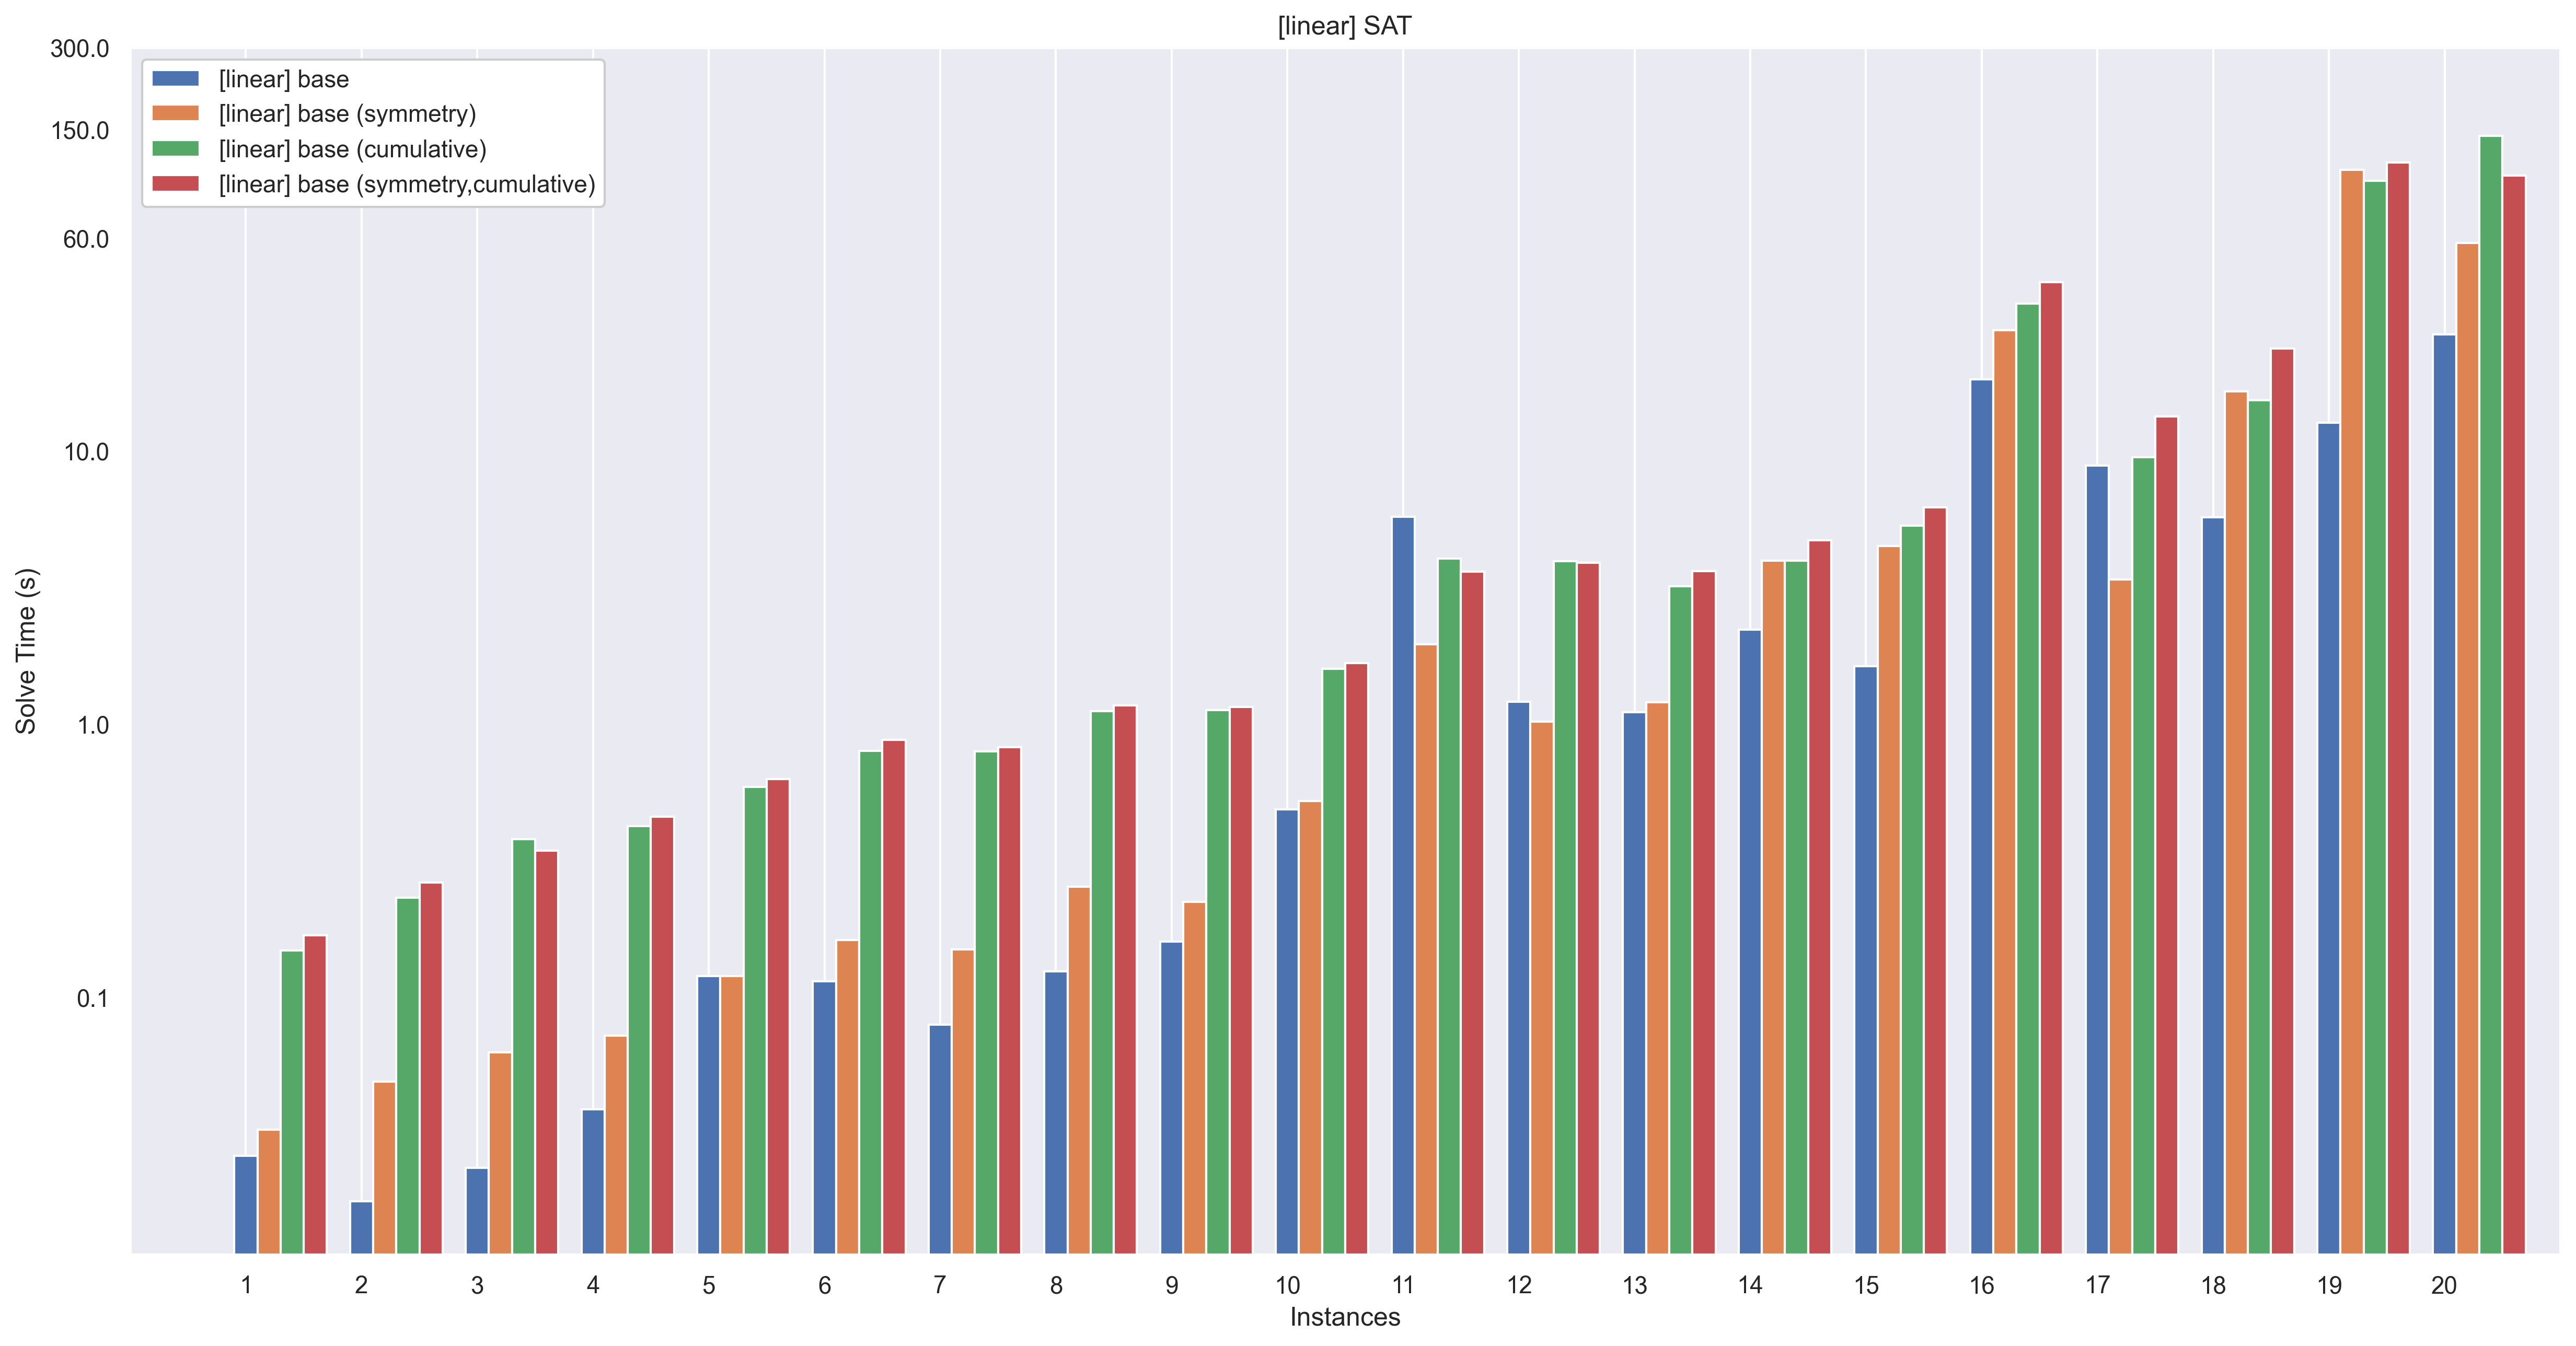
\includegraphics[width=1\textwidth]{04/results/base_linear1.png}
    \caption{
      SAT Results obtained with Base model - linear search - instances [1,20]
    }
    \label{fig:SAT_results_base_linear1}
  \end{figure}
  \begin{figure}[H]
    \centering
    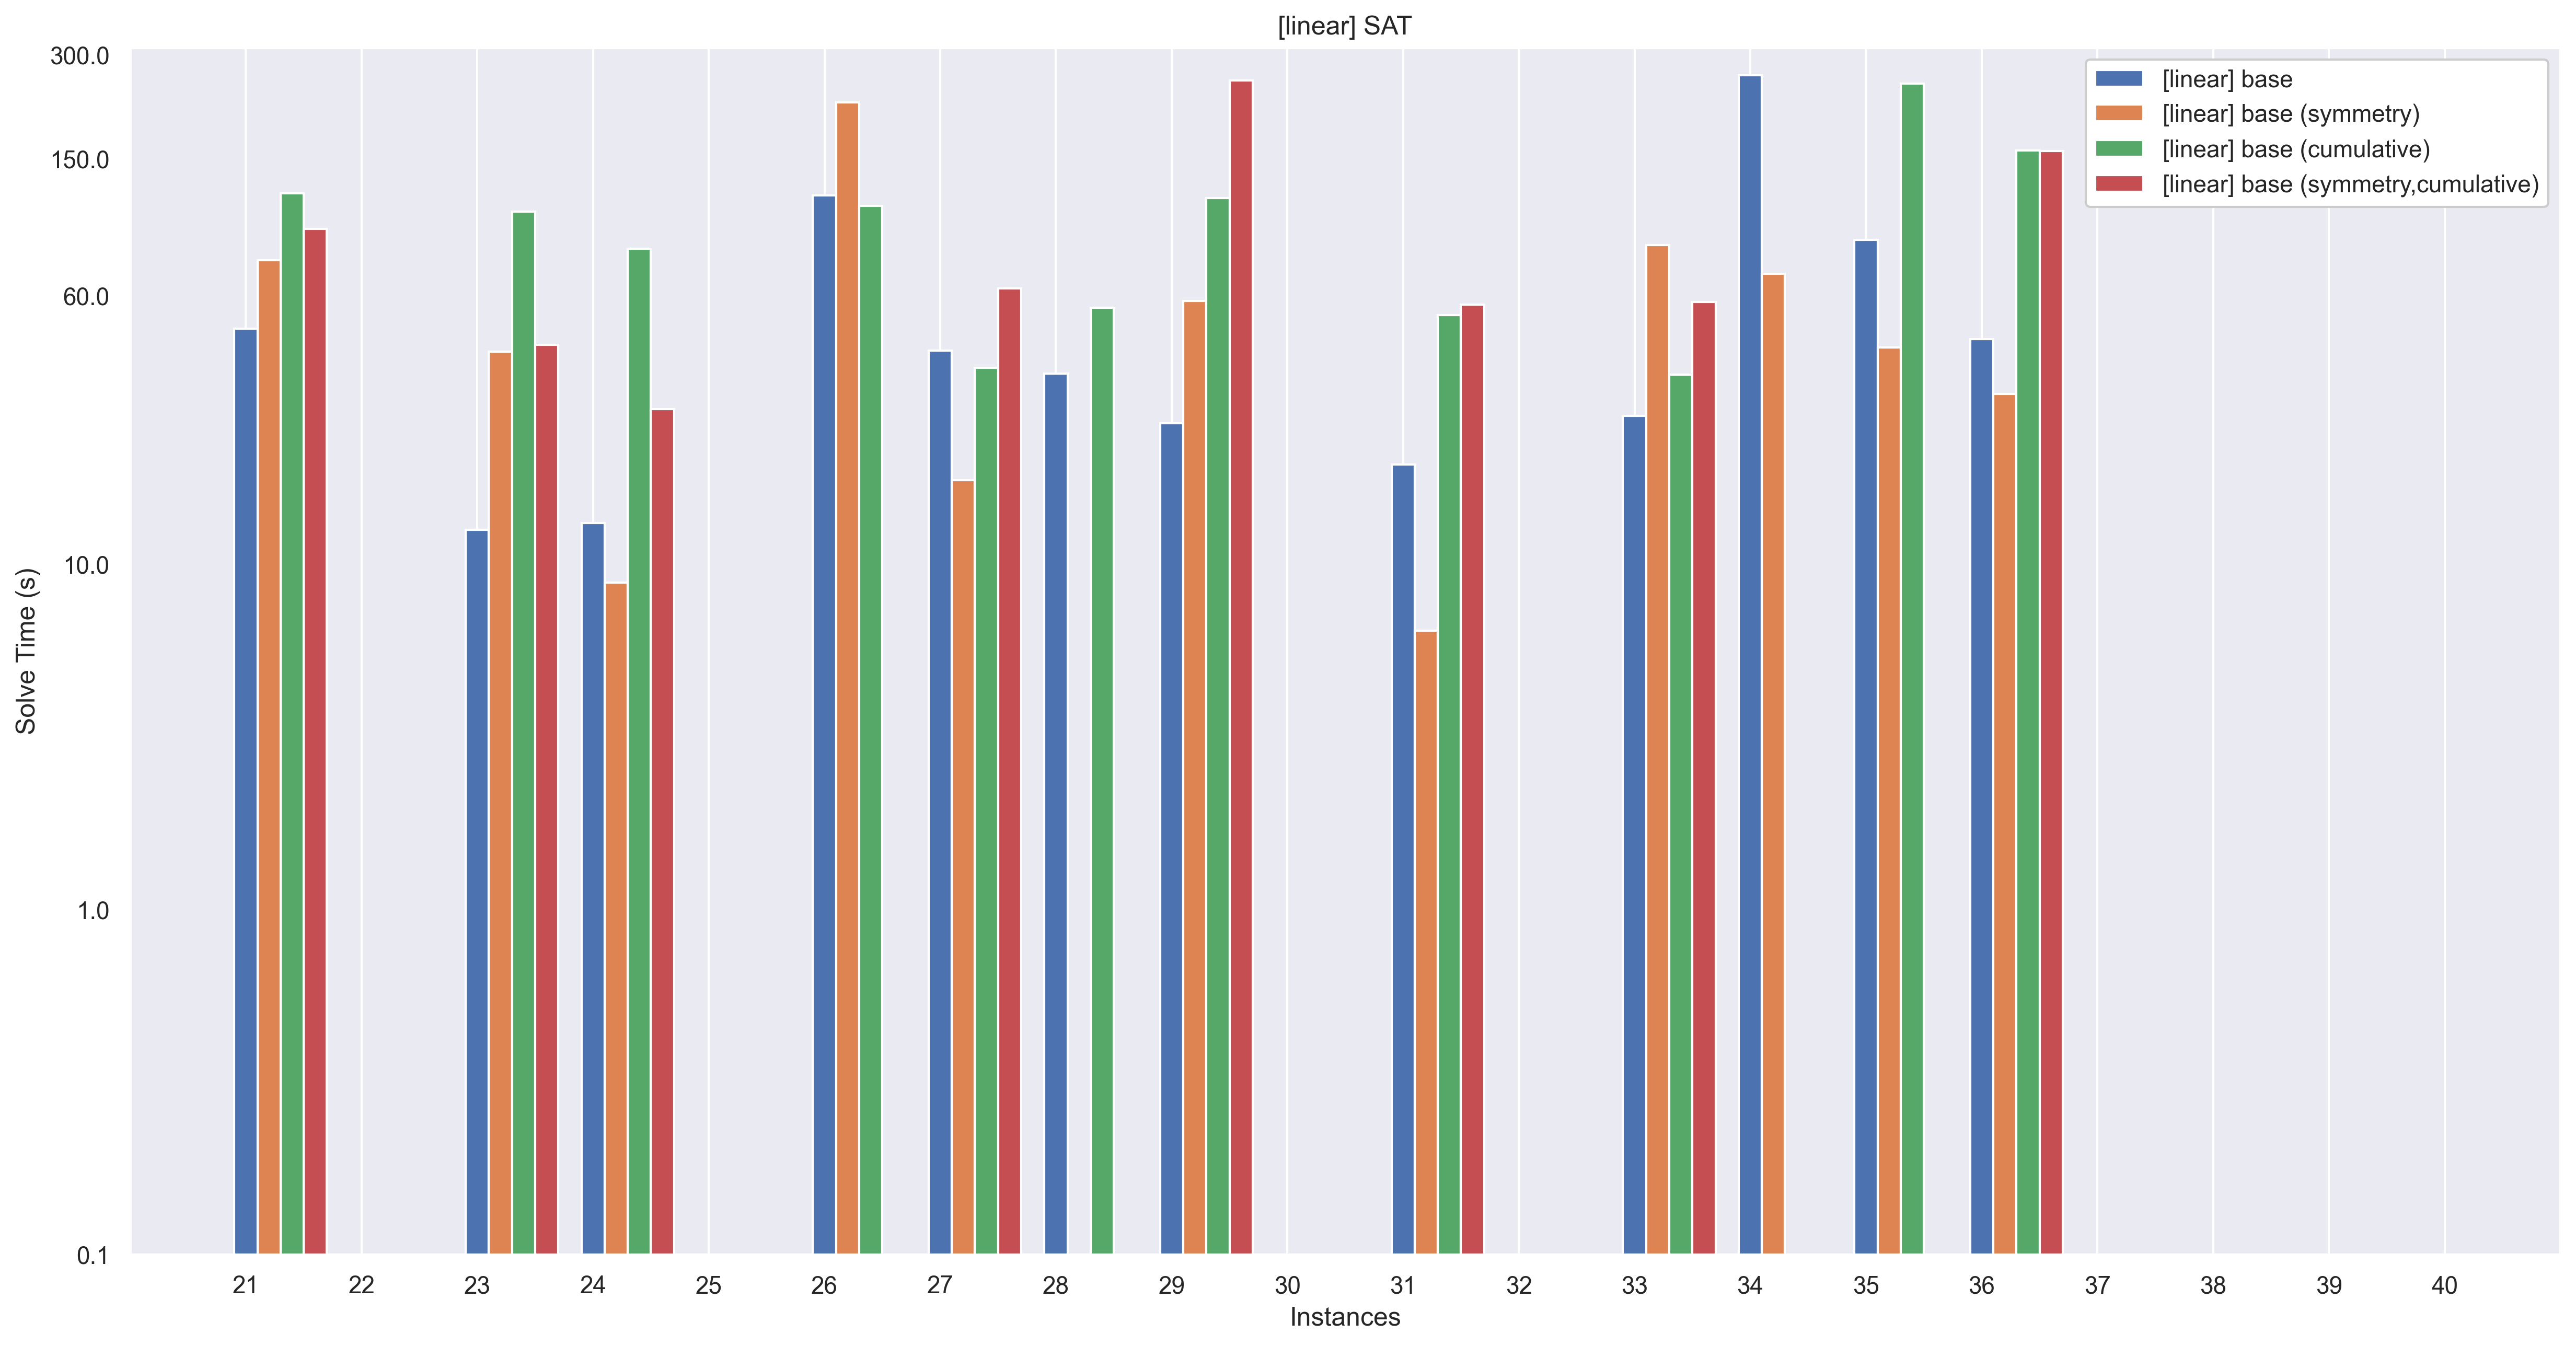
\includegraphics[width=1\textwidth]{04/results/base_linear2.png}
    \caption{
      SAT Results obtained with Base model - linear search - instances [21,40]
    }
    \label{fig:SAT_results_base_linear2}
  \end{figure}    

  \begin{figure}[H]
    \centering
    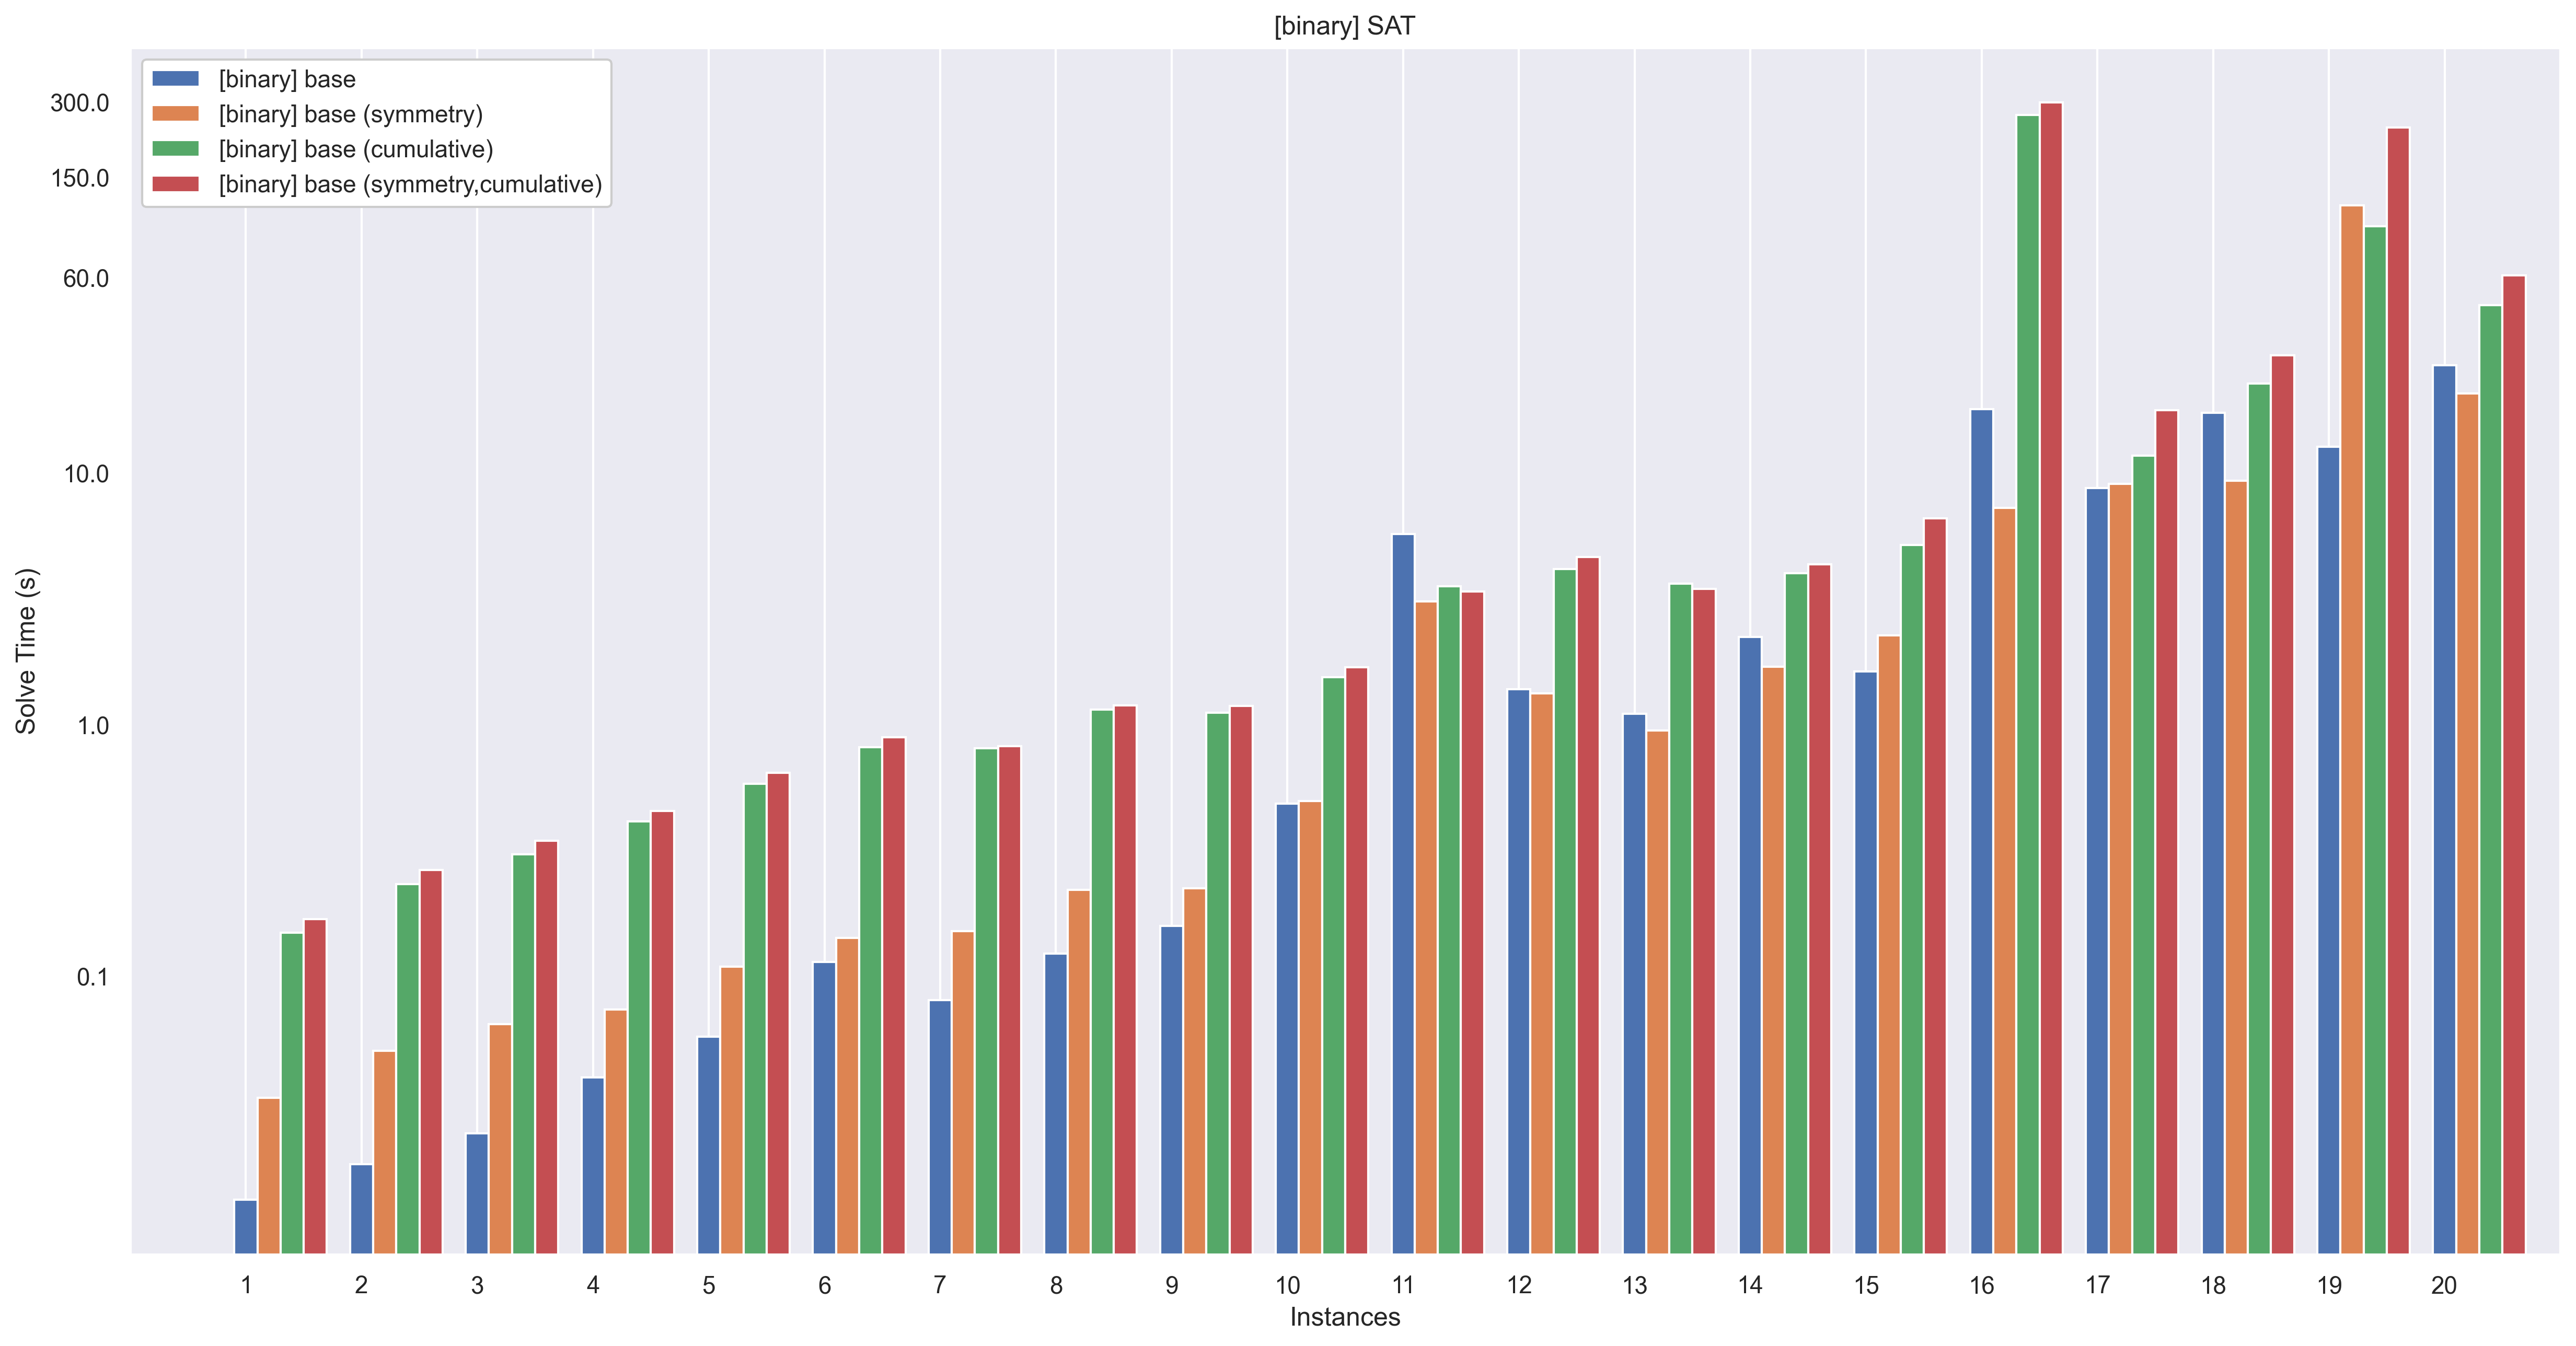
\includegraphics[width=1\textwidth]{04/results/base_binary1.png}
    \caption{
      SAT Results obtained with Base model - Binary search - instances [1,20]
    }
    \label{fig:SAT_results_base_binary1}
  \end{figure}
  \begin{figure}[H]
    \centering
    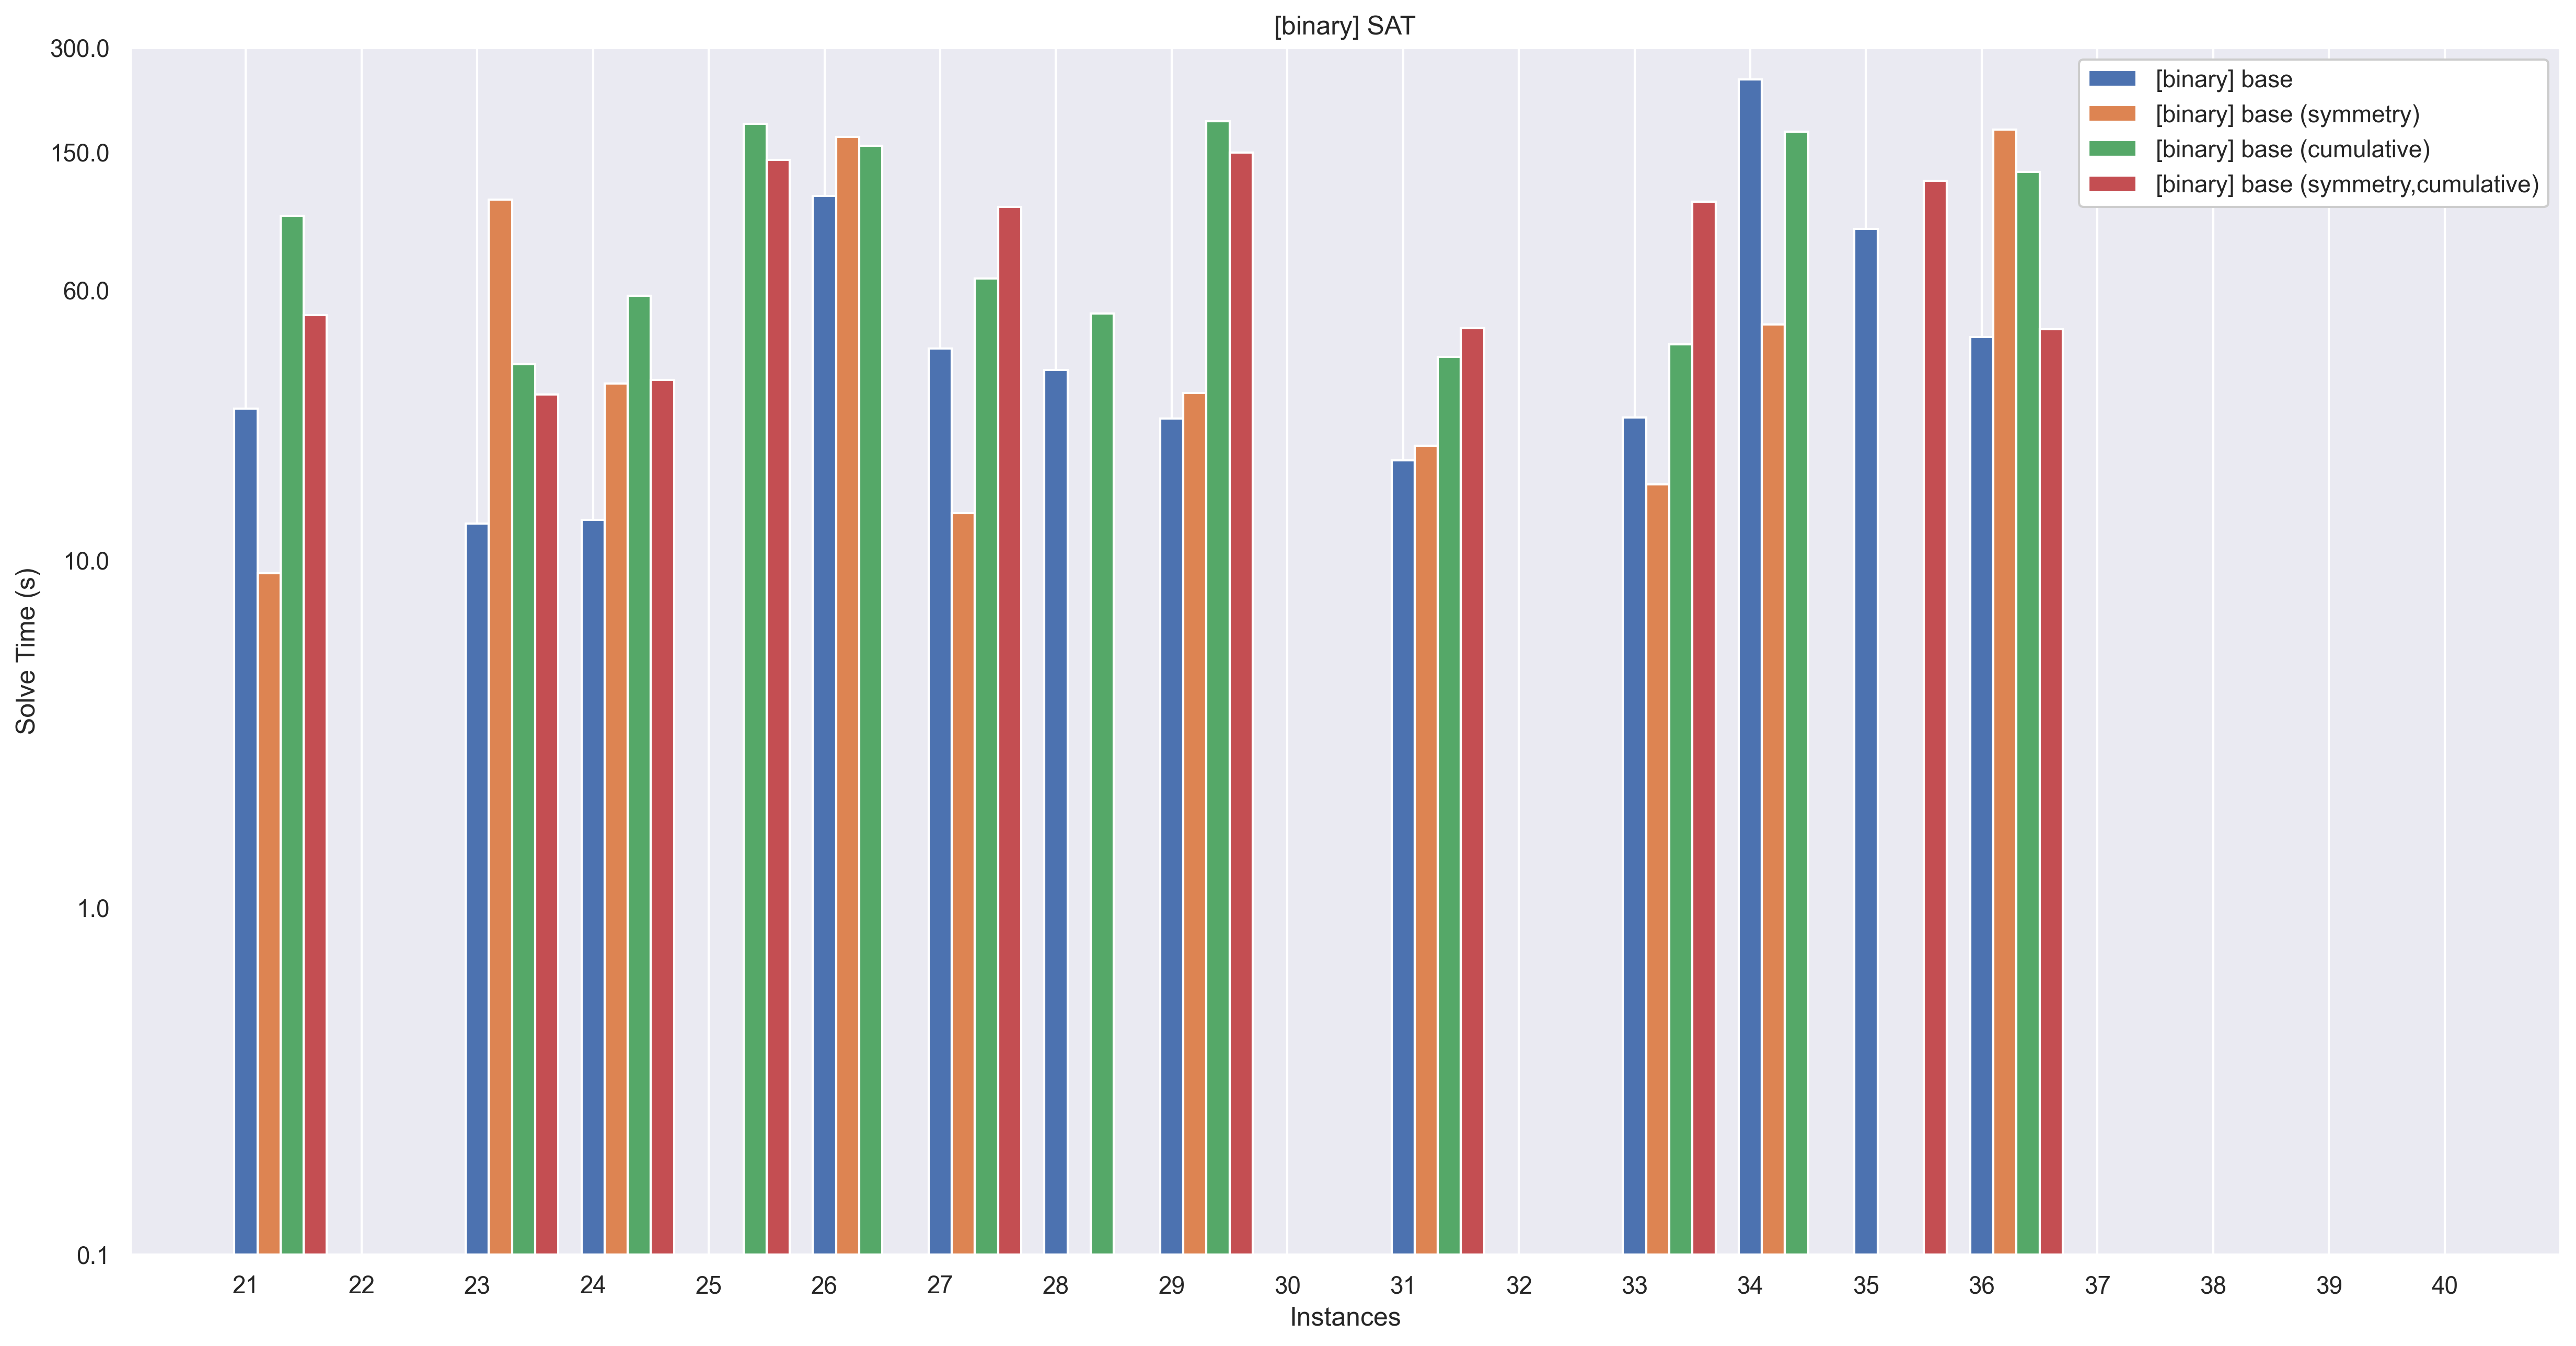
\includegraphics[width=1\textwidth]{04/results/base_binary2.png}
    \caption{
      SAT Results obtained with Base model - binary search - instances [21,40]
    }
    \label{fig:SAT_results_base_binary2}
  \end{figure} 
  
  %

  \paragraph{Rotation model}
  The results obtained with the Rotation model are in Figures [\ref{fig:SAT_results_rotation_linear1}, \ref{fig:SAT_results_rotation_linear2}]
  for linear search and in Figures [\ref{fig:SAT_results_rotation_binary1}, \ref{fig:SAT_results_rotation_binary2}] for binary search.
  
  \begin{figure}[H]
    \centering
    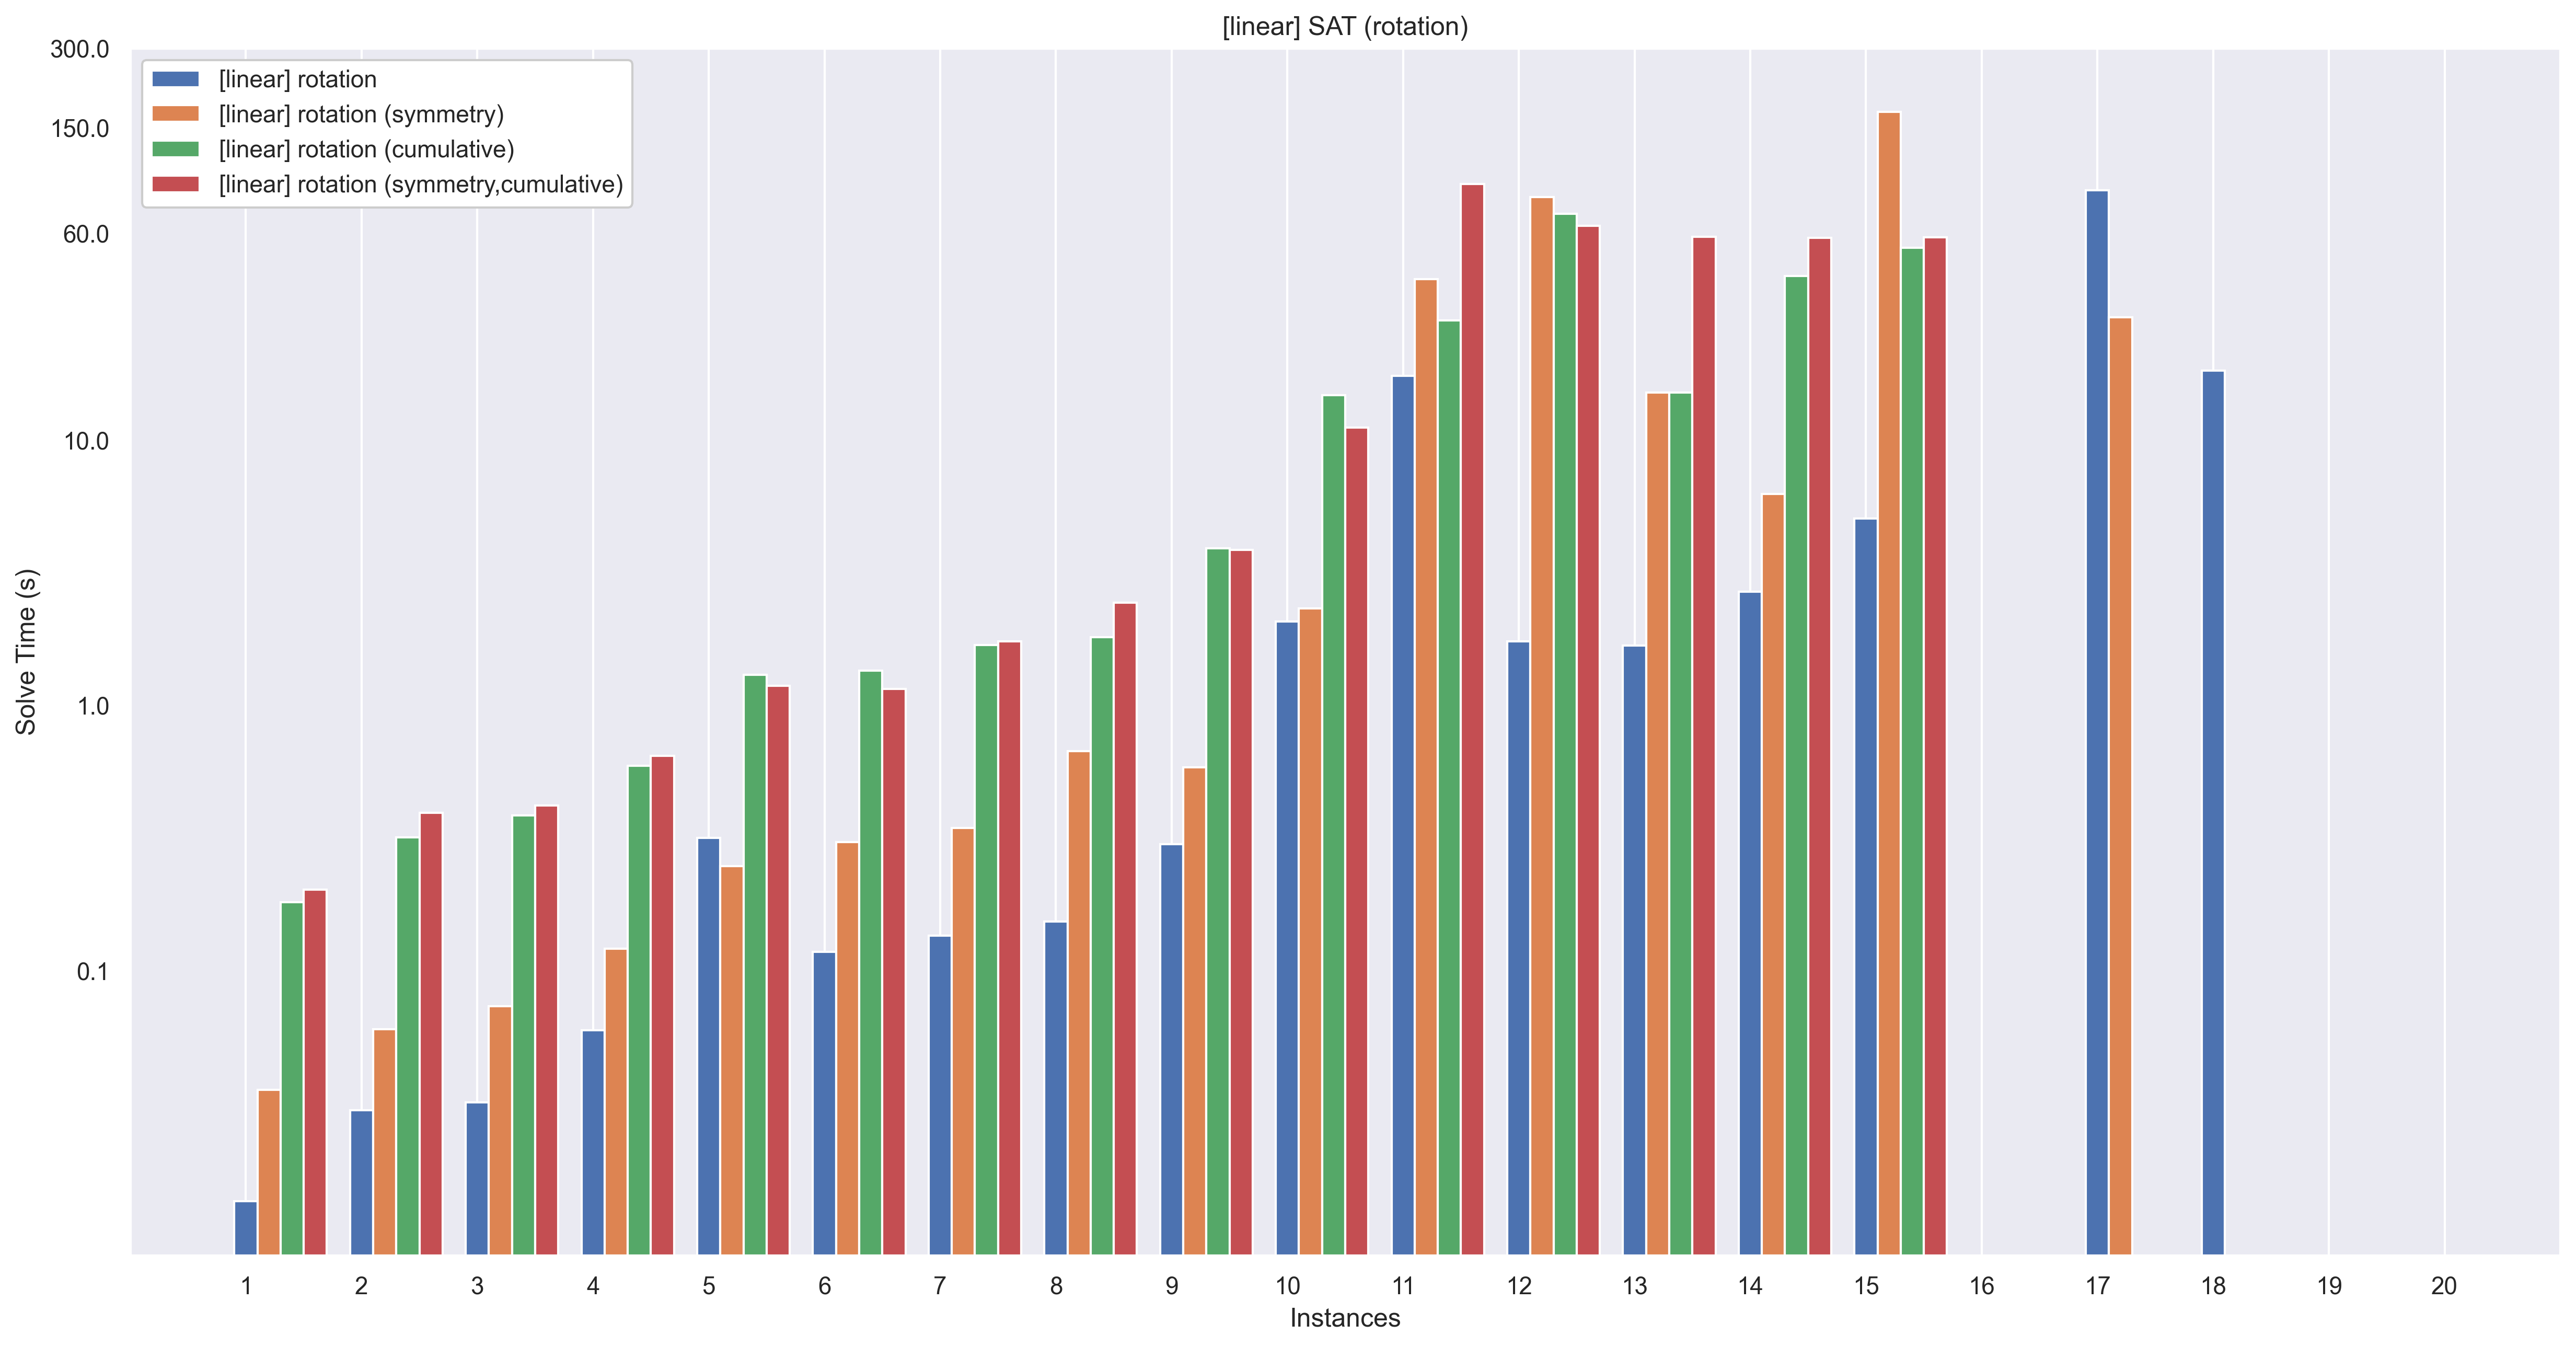
\includegraphics[width=1\textwidth]{04/results/rotation_linear1.png}
    \caption{
      SAT Results obtained with Rotation model - linear search - instances [1,20]
    }
    \label{fig:SAT_results_rotation_linear1}
  \end{figure}
  %
  \begin{figure}[H]
    \centering
    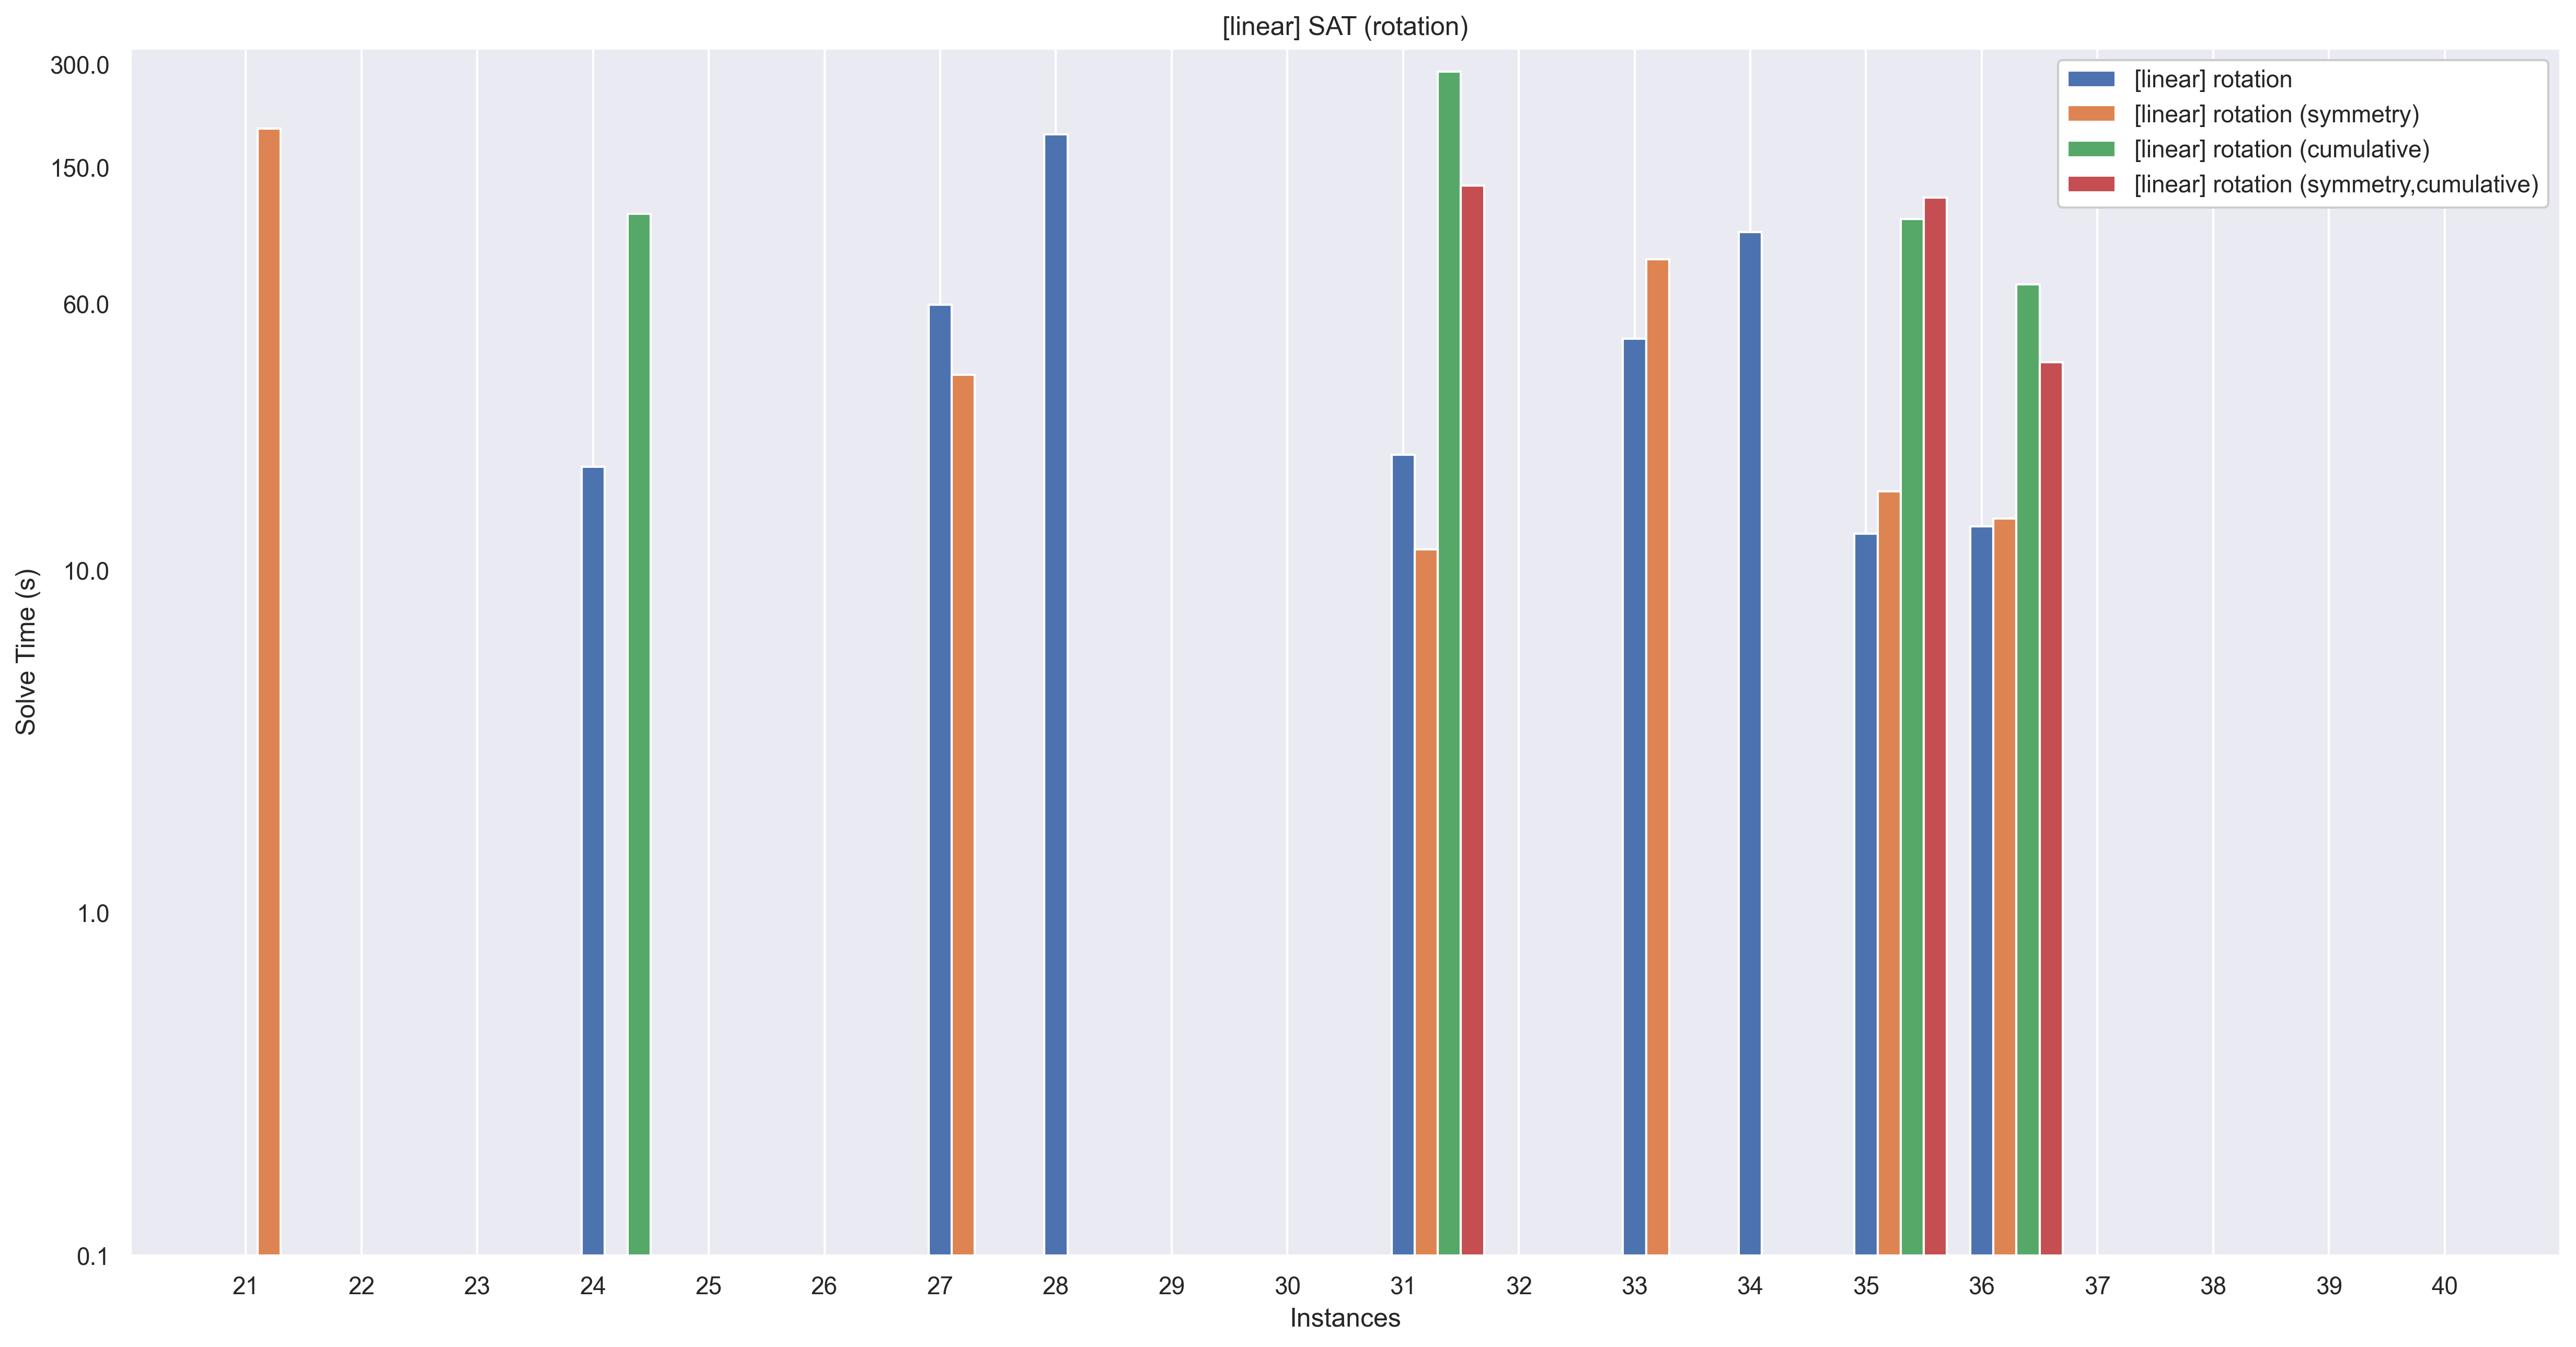
\includegraphics[width=1\textwidth]{04/results/rotation_linear2.png}
    \caption{
      SAT Results obtained with Rotation model - linear search - instances [21,40]
    }
    \label{fig:SAT_results_rotation_linear2}
  \end{figure}   
  % 
  \begin{figure}[H]
    \centering
    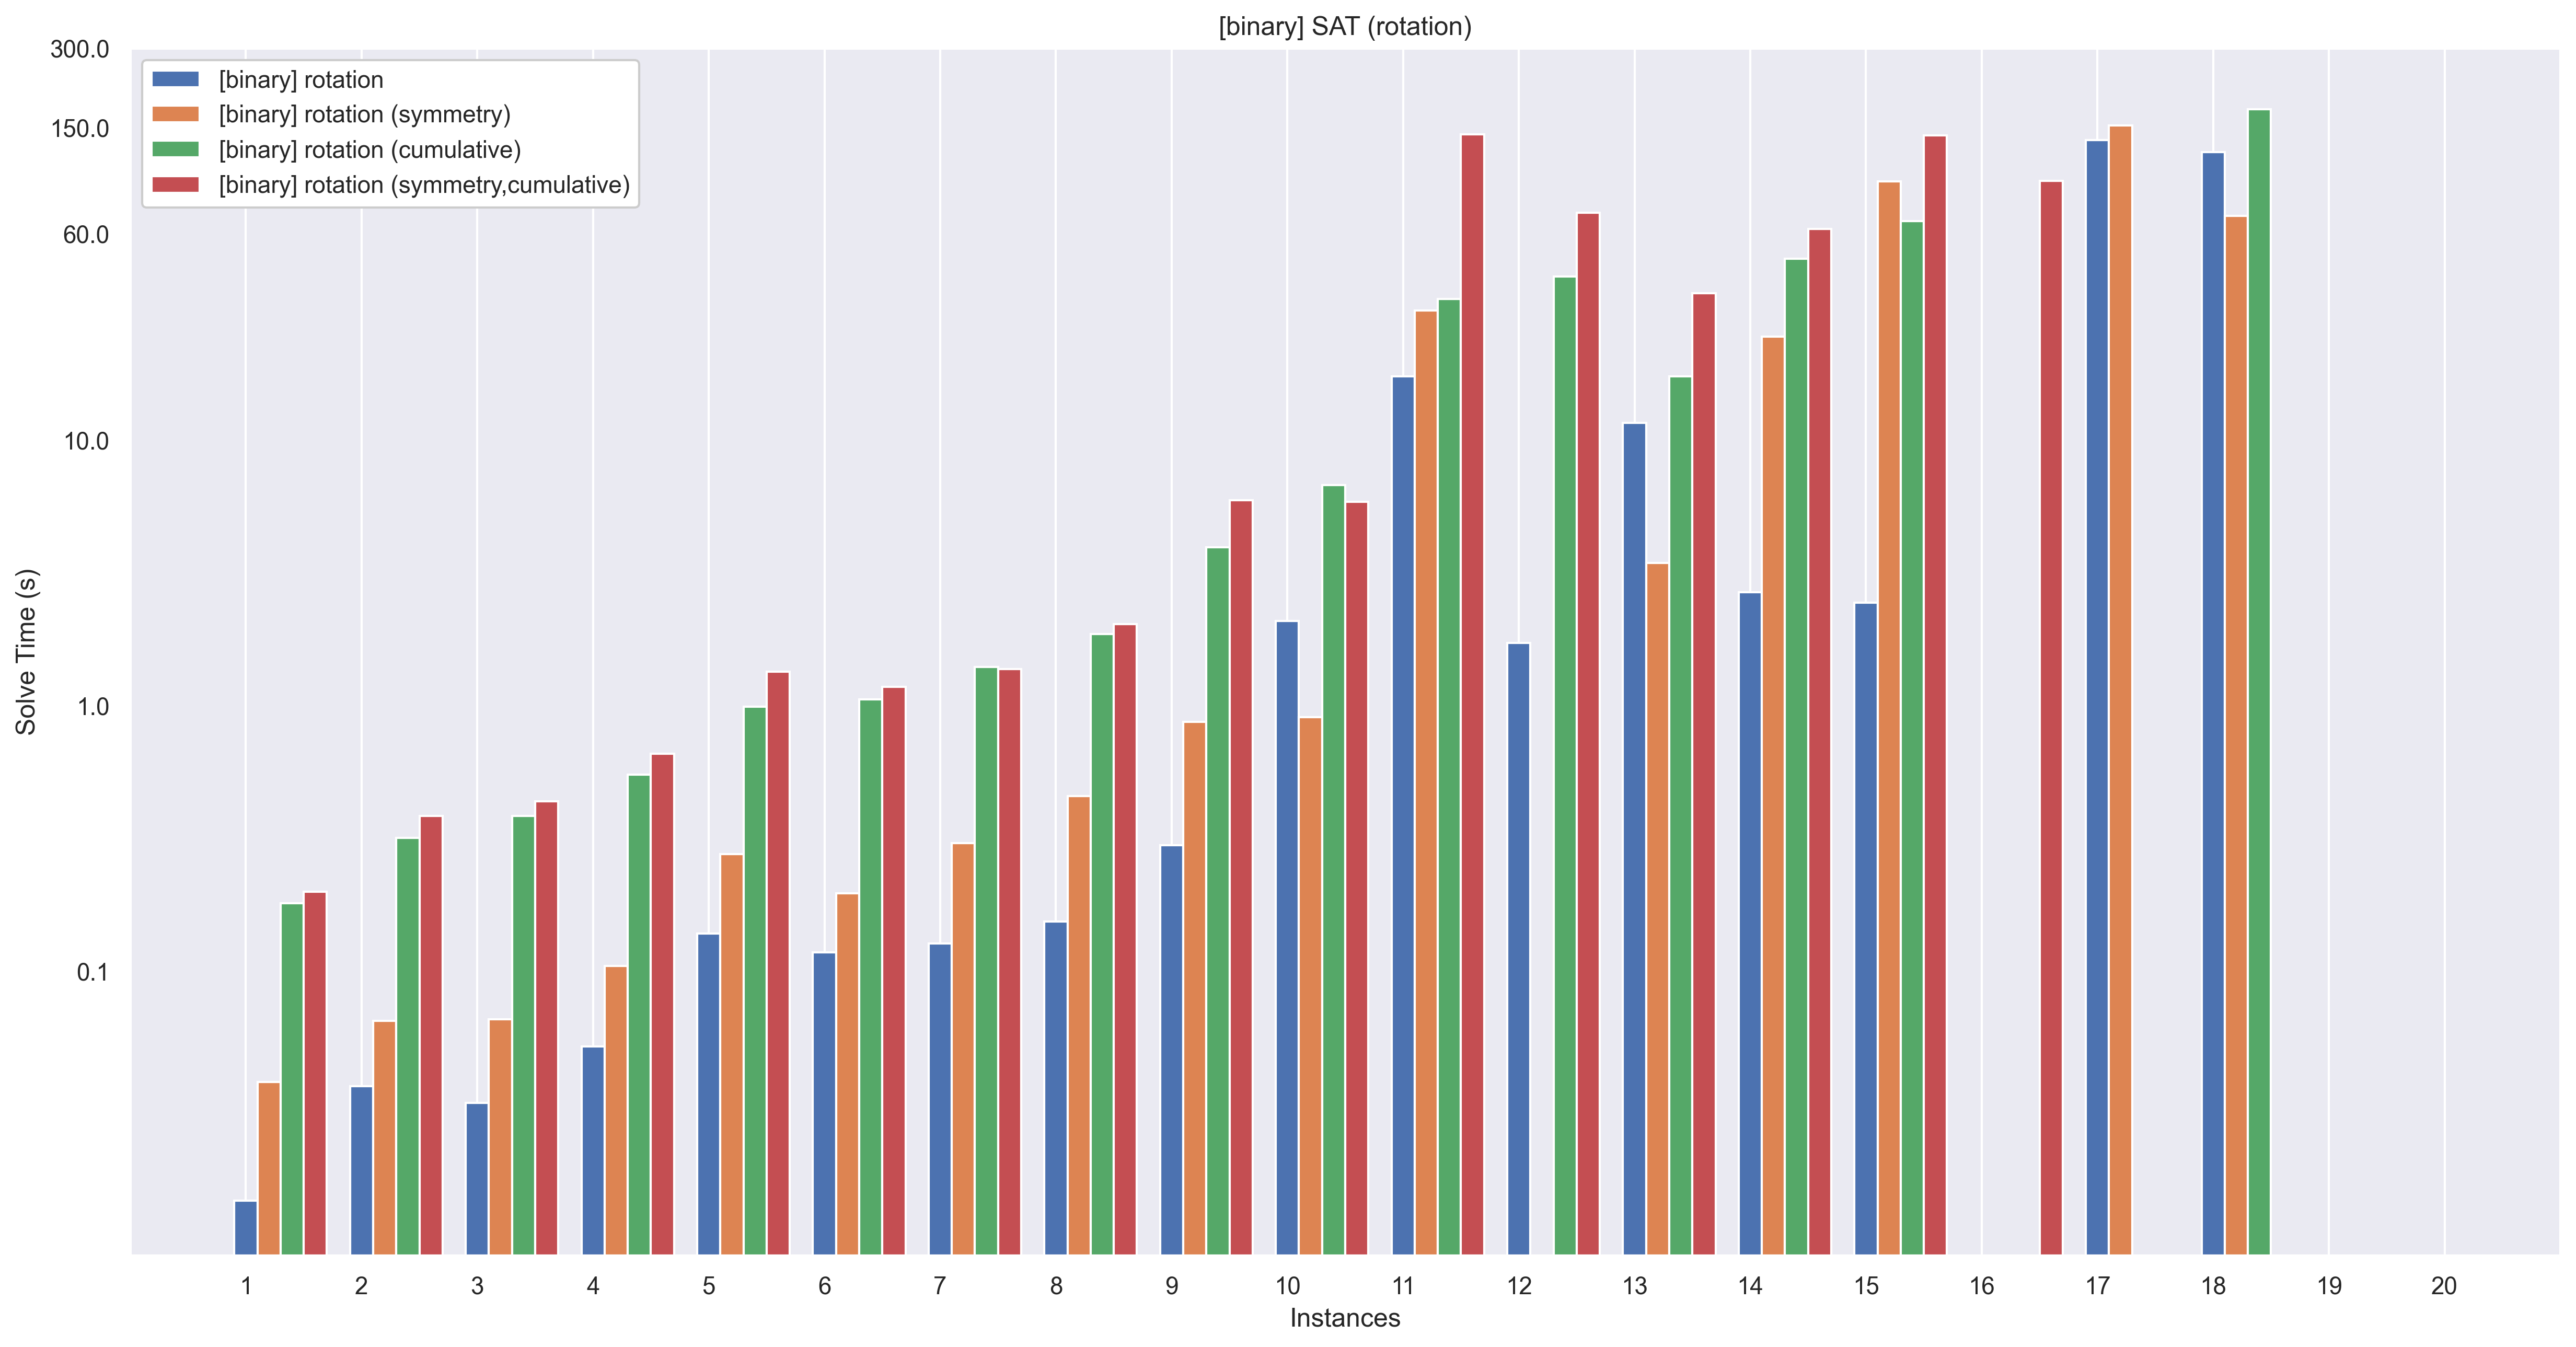
\includegraphics[width=1\textwidth]{04/results/rotation_binary1.png}
    \caption{
      SAT Results obtained with Rotation model - binary search - instances [1,20]
    }
    \label{fig:SAT_results_rotation_binary1}
  \end{figure}
  %
  \begin{figure}[H]
    \centering
    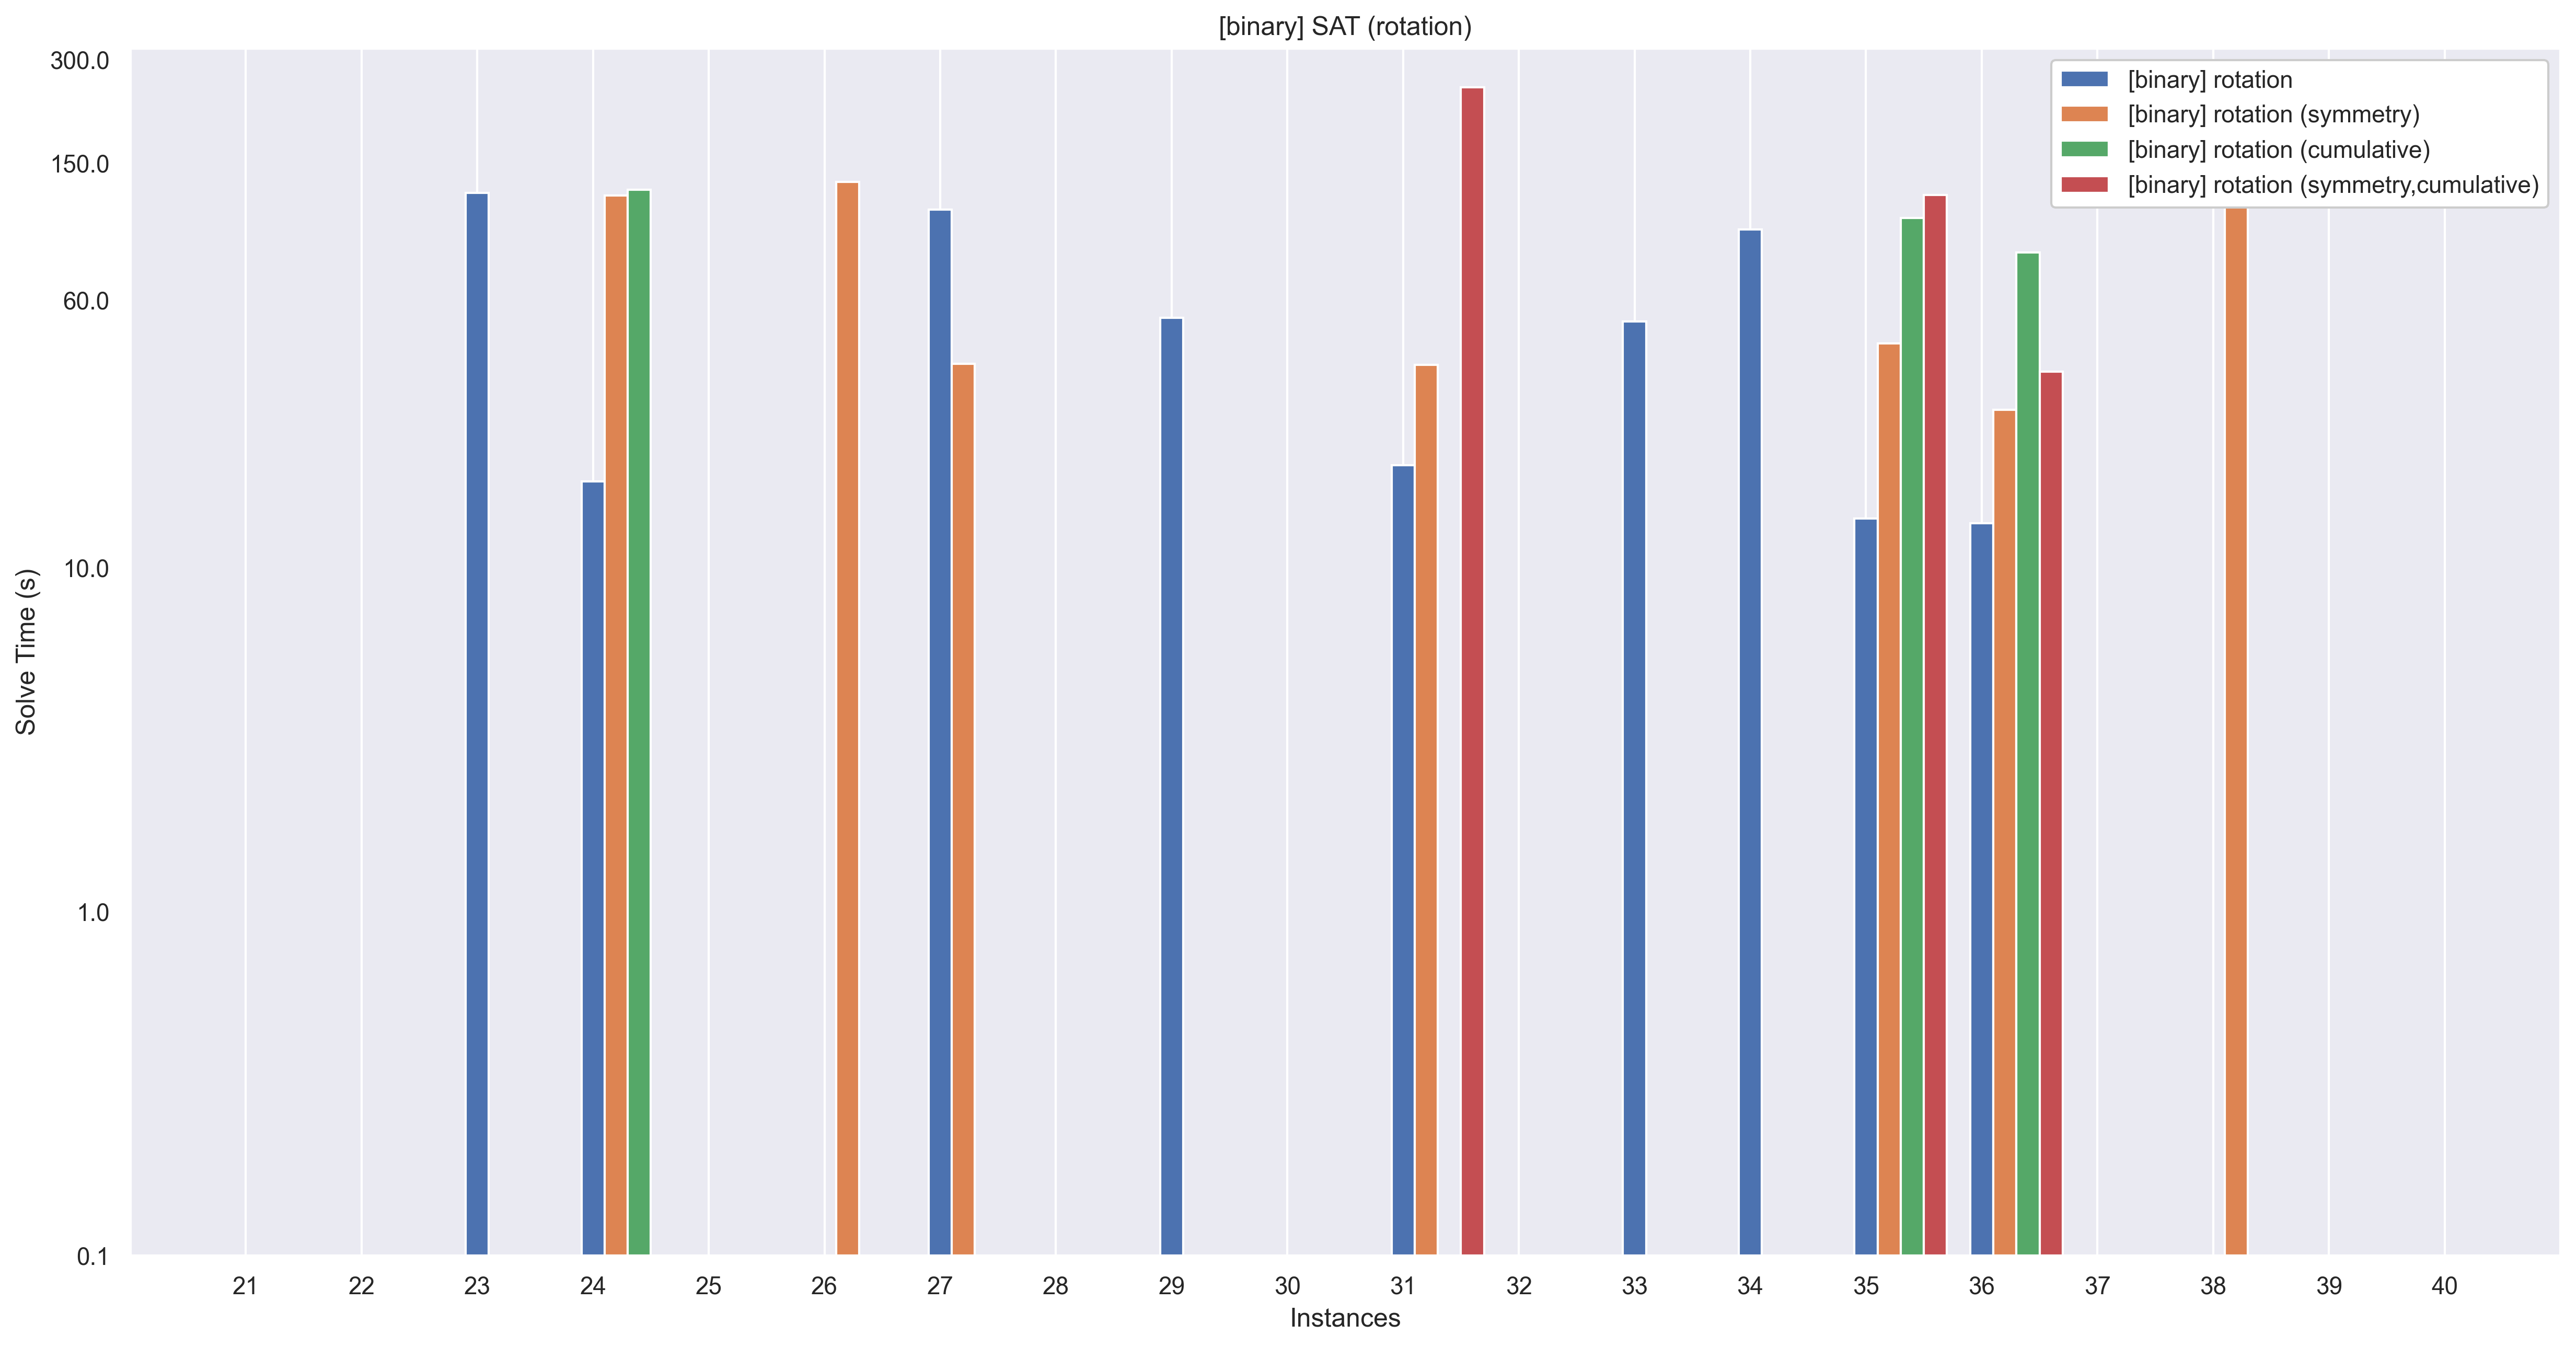
\includegraphics[width=1\textwidth]{04/results/rotation_binary2.png}
    \caption{
      SAT Results obtained with Rotation model - binary search - instances [21,40]
    }
    \label{fig:SAT_results_rotation_binary2}
  \end{figure}


